\documentclass{article}
\usepackage[utf8]{inputenc}
\usepackage{graphicx}
\usepackage{amsmath}


\title{Hw2}
\author{Konstantios Konstantinidis 2546\\
        Nikolaos Stavrinos 2631}
\date{December 2020}

\begin{document}

\maketitle
\section{.}
In order to find the minimum of the function ${\displaystyle f(\mathbf {x} )=\mathbf {x} ^{\mathsf {T}}\mathbf {A} \mathbf {x} ,\qquad \mathbf {x} \in \mathbf {R} ^{n}.}$
we need to find what value sets its derivative to zero,that's where we will use the Conjugate Gradient (Fletcher-Reeves)\\
${\displaystyle \nabla f(\mathbf {x} )=\mathbf {A} \mathbf {x} =0\,.}\\
\left[\begin{array}{cc} {3} & {1} \\ {1} & {2} \end{array}\right]\left[\begin{array}{l} {x_1} \\ {x_2} \end{array}\right]=0$\\~\\
For x1=1.5 and x2=-0.75=$>$\\
${\displaystyle \mathbf {r} _{0}={\begin{bmatrix}0\\0\end{bmatrix}}-{\begin{bmatrix}3&1\\1&2\end{bmatrix}}{\begin{bmatrix}1.5\\-0.75\end{bmatrix}}={\begin{bmatrix}-3.75\\0\end{bmatrix}}=\mathbf {p} _{0}.}$\\
${\displaystyle \alpha _{0}={\frac {\mathbf {r} _{0}^{\mathsf {T}}\mathbf {r} _{0}}{\mathbf {p} _{0}^{\mathsf {T}}\mathbf {Ap} _{0}}}={\frac {{\begin{bmatrix}-3.75&0\end{bmatrix}}{\begin{bmatrix}-3.75\\0\end{bmatrix}}}{{\begin{bmatrix}-3.75&0\end{bmatrix}}{\begin{bmatrix}3&1\\1&2\end{bmatrix}}{\begin{bmatrix}-3.75\\0\end{bmatrix}}}}={\frac {1
}{3}}.}$\\
${\displaystyle \mathbf {x} _{1}=\mathbf {x} _{0}+\alpha _{0}\mathbf {p} _{0}={\begin{bmatrix}1.5\\-0.75\end{bmatrix}}+{\frac {1}{3}}{\begin{bmatrix}-3.75\\0\end{bmatrix}}={\begin{bmatrix}0.25\\-0.75\end{bmatrix}}.}$\\
Second iteration:\\
${\displaystyle \mathbf {r} _{1}=\mathbf {r} _{0}-\alpha _{0}\mathbf {A} \mathbf {p} _{0}={\begin{bmatrix}-3.75\\0\end{bmatrix}}-{\frac {1}{3}}{\begin{bmatrix}3&1\\1&2\end{bmatrix}}{\begin{bmatrix}-3.75\\0\end{bmatrix}}={\begin{bmatrix}0\\1.25\end{bmatrix}}.}$\\
${\displaystyle \beta _{0}={\frac {\mathbf {r} _{1}^{\mathsf {T}}\mathbf {r} _{1}}{\mathbf {r} _{0}^{\mathsf {T}}\mathbf {r} _{0}}}={\frac {{\begin{bmatrix}0&1.25\end{bmatrix}}{\begin{bmatrix}0\\1.25\end{bmatrix}}}{{\begin{bmatrix}-3.75&0\end{bmatrix}}{\begin{bmatrix}-3.75\\0\end{bmatrix}}}}={\frac {1}{9}}.}$\\
${\displaystyle \mathbf {p} _{1}=\mathbf {r} _{1}+\beta _{0}\mathbf {p} _{0}={\begin{bmatrix}0\\1.25\end{bmatrix}}+{\frac{1}{9}}{\begin{bmatrix}-3.75\\0\end{bmatrix}}={\frac {1}{3}}{\begin{bmatrix}-1.25\\3.75\end{bmatrix}}.}$\\
${\displaystyle \alpha _{1}={\frac {\mathbf {r} _{1}^{\mathsf {T}}\mathbf {r} _{1}}{\mathbf {p} _{1}^{\mathsf {T}}\mathbf {Ap} _{1}}}=9*{\frac {{\begin{bmatrix}0&1.25\end{bmatrix}}{\begin{bmatrix}0\\1.25\end{bmatrix}}}{{\begin{bmatrix}-1.25&3.75\end{bmatrix}}{\begin{bmatrix}3&1\\1&2\end{bmatrix}}{\begin{bmatrix}-1.25\\3.75\end{bmatrix}}}}=0.6.}$\\
${\displaystyle \mathbf {x} _{2}=\mathbf {x} _{1}+\alpha _{1}\mathbf {p} _{1}={\begin{bmatrix}0.25\\-0.75\end{bmatrix}}+0.2{\begin{bmatrix}-1.25\\3.75\end{bmatrix}}={\begin{bmatrix}0\\0\end{bmatrix}}.}$\\~\\
In order to find the minimum of the function ${\displaystyle f(\mathbf {x} )=3w_1^2+2w_2^2+2w_1w_2}$with gradient descent\\
${\displaystyle \nabla f(\mathbf {x} )=\left[\begin{array}{cc} {6w_1 + 2w_2} \\ {2w_1 + 4w_2} \end{array}\right]\ =0\,.}$\\
$(w_1(1),w_2(1))=(w_1(0),w_2(0))-t_0\nabla f((w_1(0),w_2(0) )$\\
To find t0 we need to find the minimum of the function $\theta(t)=f(w_1(0),w_2(0))-t_0\nabla f((w_1(0),w_2(0) )$\\
$\theta'(t)= -\nabla f((w_1(0), w_2(0)) - t\nabla f(w_1(0), w_2(0)))^T\nabla f(w_1(0), w_2(0))=f(w_1(0),w_2(0))-t_0\nabla f(1.5-0.75t,-0.75+3t)^T*\nabla f(7.5,-3)=-38.25+283.5t$\\
That has to equal to zero,so t=0.135\\
So $(w_1(1),w_2(1))=(1.5,-0.75)-0.135*(7.5,-3)=(1.5-1.012,-0.75+0.405)=(0.488,-0.345)$\\
Second iteration:\\
$\theta '(t)==f(w_1(1),w_2(1))-t_0\nabla f(1.5-0.75t,-0.75+3t)^T*\nabla f(7.5,-3)=-3.762+13.98*t$\\
That has to equal to zero,so t=0.269\\
So $(w_1(2),w_2(2))=(0.488,-0.345)-0.269*(1.608,-0.404)=(0.055,-0.236)$\\
which will also converge to (0,0) as well.

\newpage
\section{.}
\begin{figure}[htp]
    \centering
    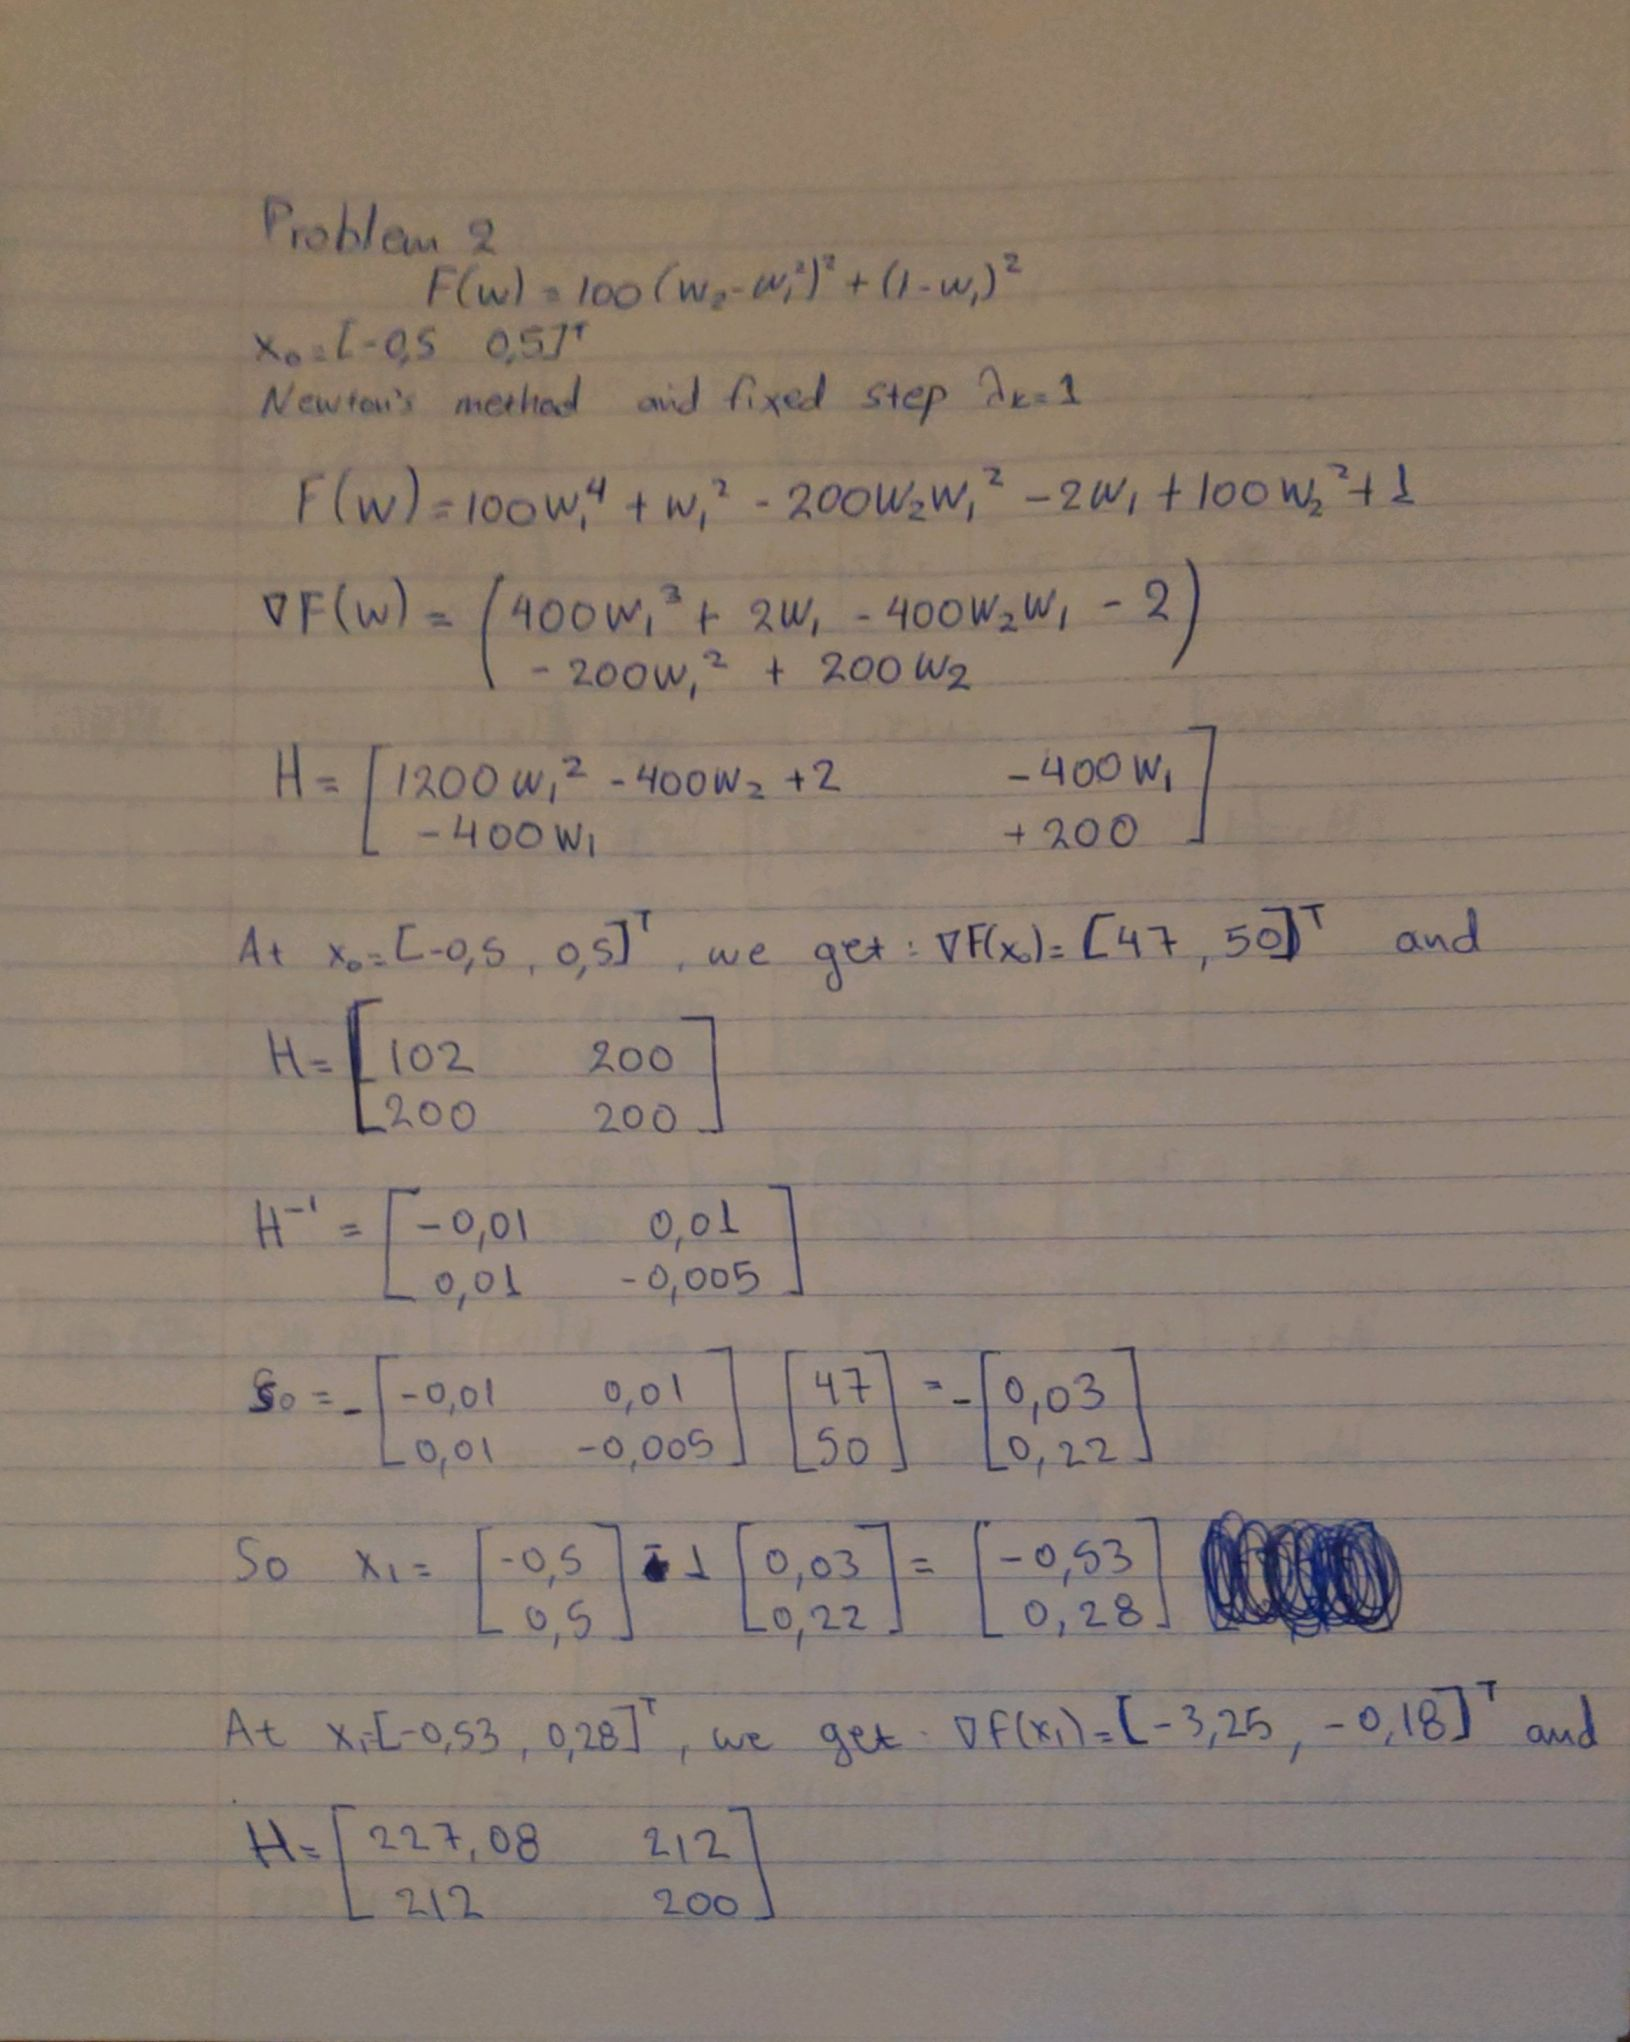
\includegraphics[width=11cm]{photos/2_1.jpg}
    \caption{}
    \label{}
\end{figure}
\newpage
\begin{figure}[htp]
    \centering
    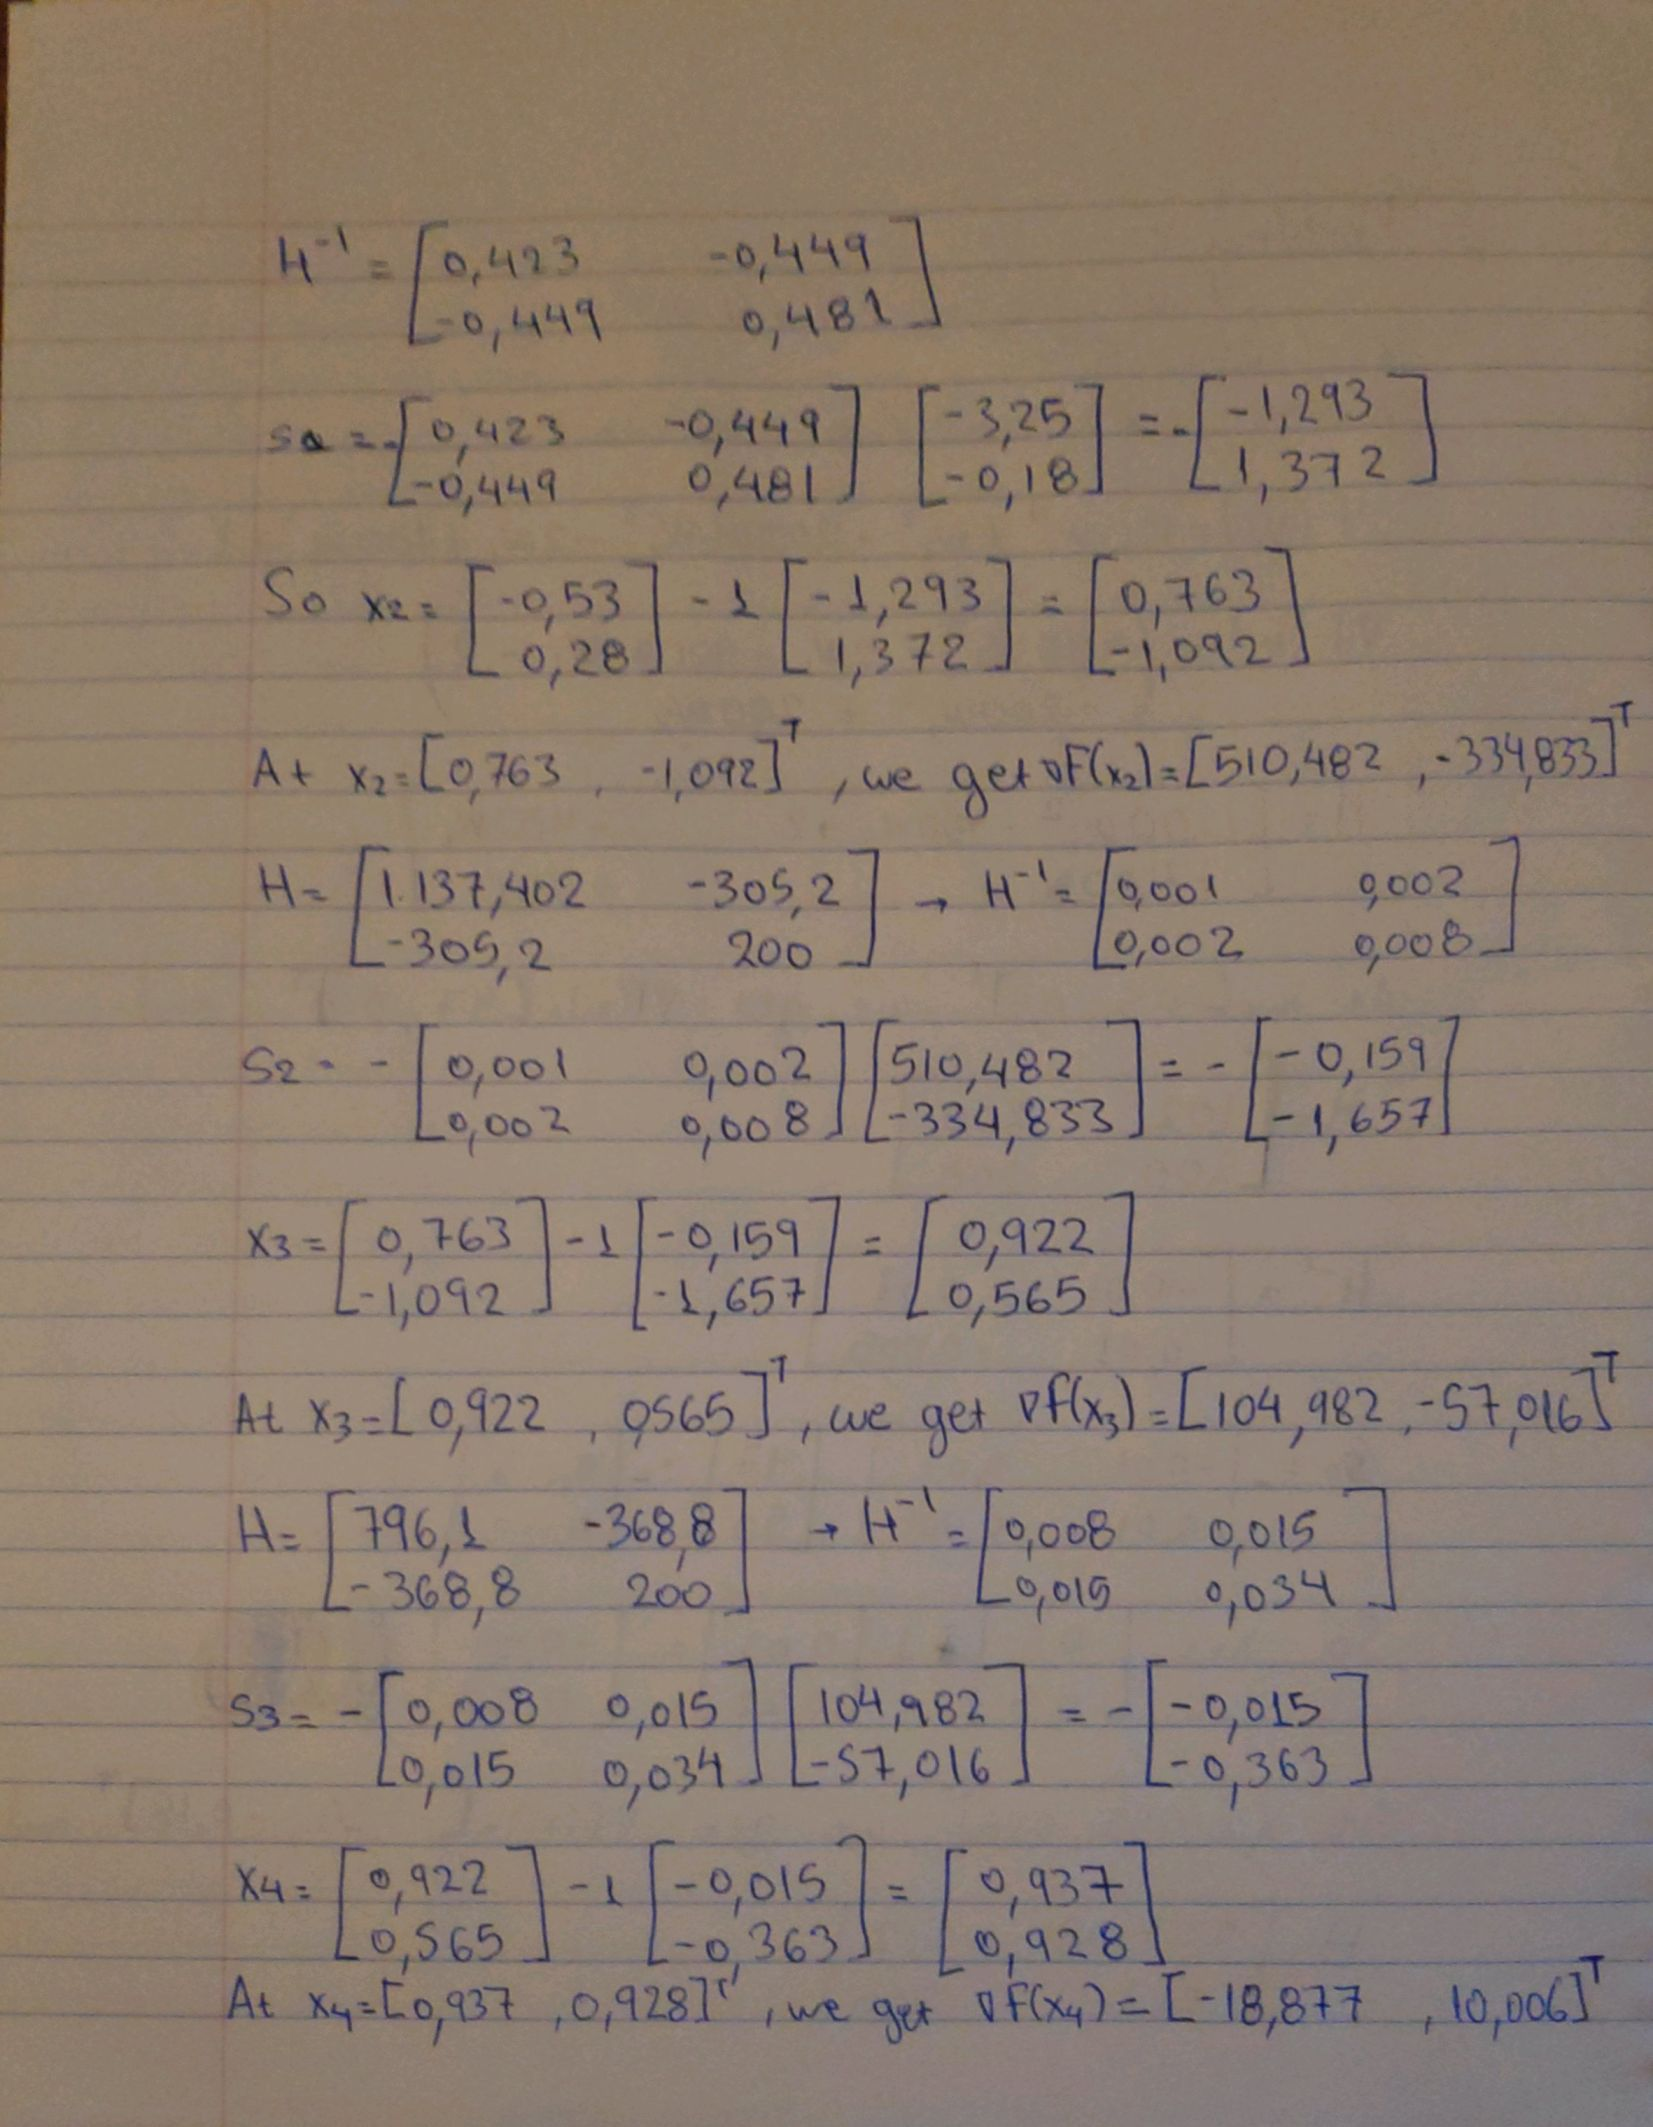
\includegraphics[width=11cm]{photos/2_2.jpg}
    \caption{}
    \label{}
\end{figure}
\newpage
\begin{figure}[htp]
    \centering
    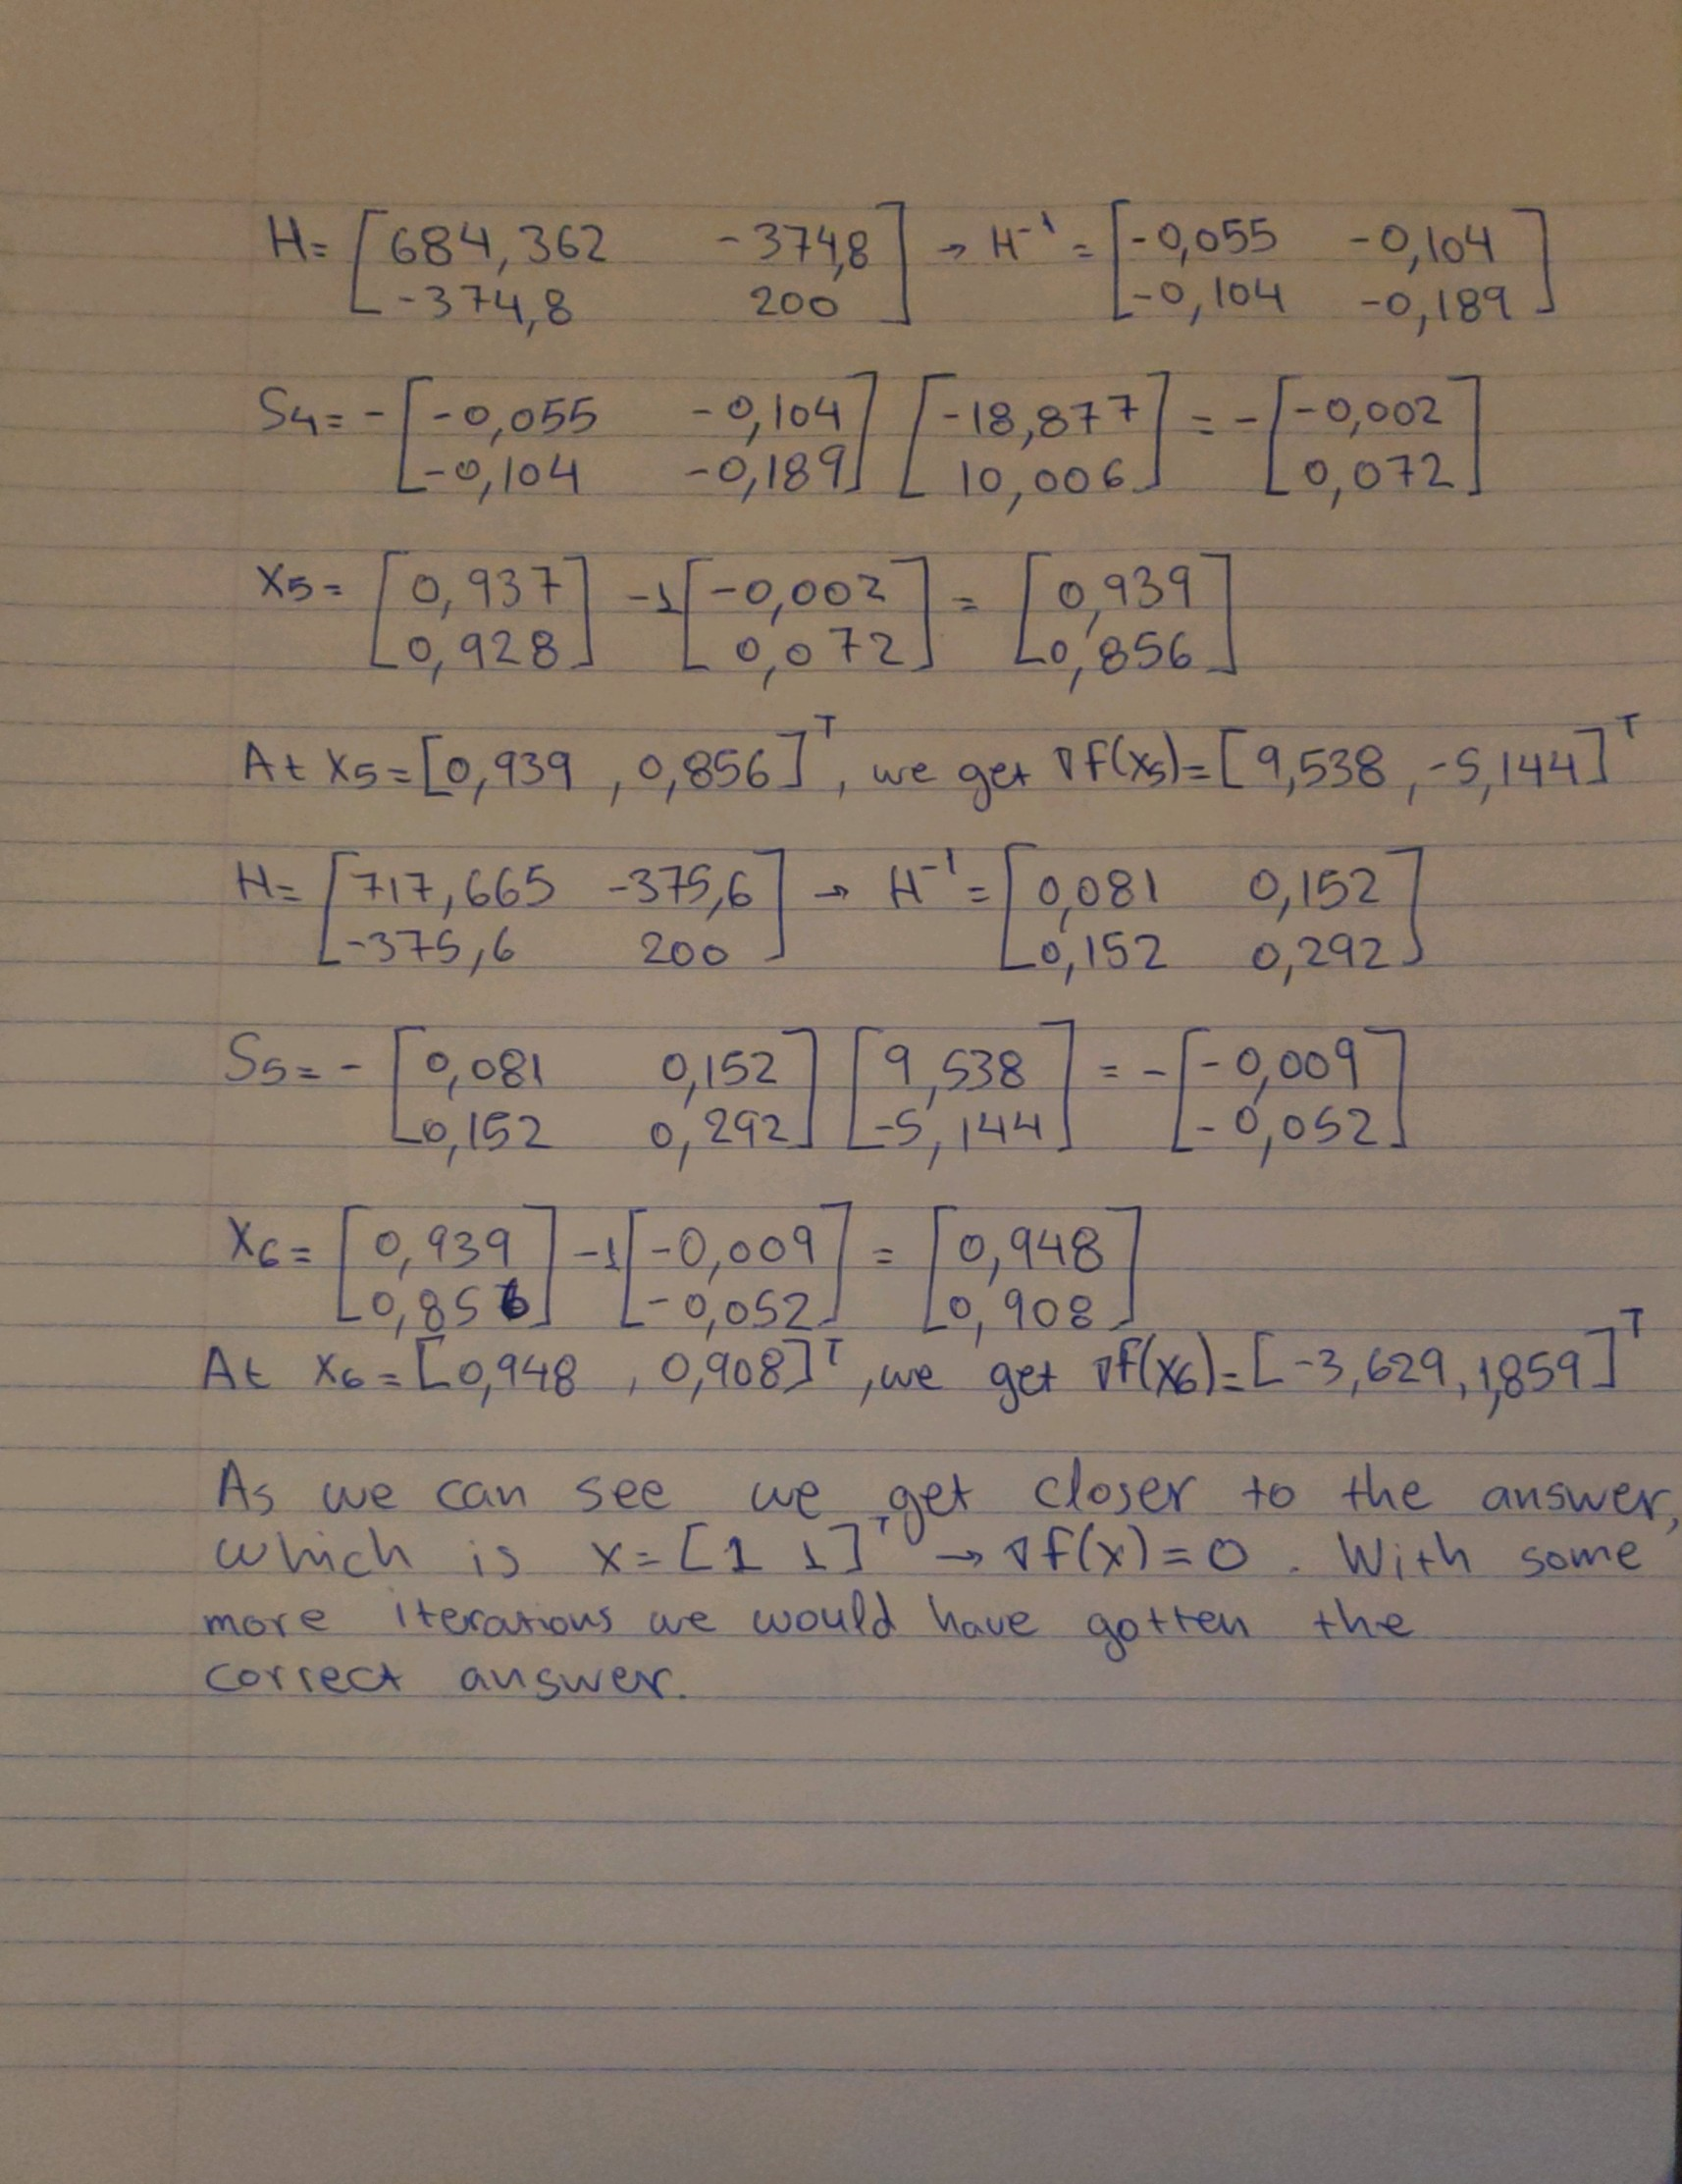
\includegraphics[width=10cm]{photos/2_3.jpg}
    \caption{}
    \label{}
\end{figure}
\newpage
\section{.}

3.
Feed-Forward Phase:

 



Compute Error:
 
a1 = (-2 * 1 + 1 * 1)3 = -1
a2 = (1 * 1  -(2 * 1))2 = 1	(2)
 


 


Backpropagation:
 Sensitivities:
 
error = 0 - output = 0 - 1 =- 1	(3)



s2 = -2Ft2’(n2)(t - a) = -4(-1) (e) = -4\\
s1 = F’1(n1)(W 2)T s2 = 3(n1 )2* 1 *(-4) = -12	(4)
 
Update weights and biases:

W 2(1) = W 2(0) - a * s2(a1)T  = 1 - 1 * (-4) * 1 = -3\\
b2(1) = b2(0) - a * s2 = -2 - 1 * (-4) = 6\\
W 1(1) = W 1(0) - a * s1(a0)T  = -2 - 1 * (-12) = 10\\
b1(1) = b1(0) - a * s1 = 1 - 1 * (-12) = 13\\
 
\section{.}
$
H1(1)=0.1*1+0.3*4+0.5*5+0.5=4.3\\
H2(1)=0.2*1+0.4*4+0.6*5+0.5=5.3\\
\\
Sigmoid(H1(1))=1/(1+e^{-4.3})=0.986\\
Sigmoid(H2(1))= 1/(1+e^{-5.3})=0.995\\
\\
O1=0.7*0.986+0.9*0.995+0.5=2.085\\
O2=0.8*0.986+0.1*0.995+0.5=1.338\\
\\
Sigmoid(O1(1))=0.889\\
Sigmoid(O2(1))=0.792\\
\\
E1=t1-0.889=0.1-0.889=-0.789\\
E2=t2-0.889=0.05-0.792=-0.749 \\
Sigmoid(x)=1/(1+e^{-x})=>Sigmoid'(x)=\frac{d}{dx}(1/(1+e^{-x})=e^{-x}/((1+e^{-x}))^2=(1-1/(1+e^{-x})*(1/(1+e^{-x})=(1-a^1)*(a^1)\\~\\
s2 = -2F'^{2}(n2)(t - a) =-2*\left[\begin{array}{cc} {a_1*(1-a_1)} & {0} \\ {0} & {a_2(1-a_2)} \end{array}\right]\left[\begin{array}{l} {-0.789} \\ {-0.749} \end{array}\right]=-2*\left[\begin{array}{cc} {0.889*(1-0.889)} & {0} \\ {0} & {0.792(1-0.792)} \end{array}\right]\left[\begin{array}{l} {-0.789} \\ {-0.75} \end{array}\right] =\left[\begin{array}{l} {0.155} \\ {0.24} \end{array}\right]\\
s1 = F'^{1}(n1)'(W^2)^T s2 = \left[\begin{array}{cc} {0.013} & {0} \\ {0} & {0.05} \end{array}\right]\left[\begin{array}{cc} {0.7} & {0.9} \\ {0.8} & {0.1} \end{array}\right]\left[\begin{array}{cc} {0.155} \\ {0.24} \end{array}\right]=\left[\begin{array}{cc} {0.0042} \\ {0.0007} \end{array}\right]
$\\
$W 2(1) = W 2(0) - a * s2(a1)T  =\left[\begin{array}{cc} {0.7} & {0.9} \\ {0.8} & {0.1} \end{array}\right]-0.01*\left[\begin{array}{cc} {0.155} \\ {0.24} \end{array}\right]\left[\begin{array}{cc} {0.986} \\ {0.995} \end{array}\right]^T\approx\left[\begin{array}{cc} {0.698} & {0.898} \\ {0.797} & {0.017} \end{array}\right]$\\
b2(1) = b2(0) - a * s2 = -2 - 1 * (-4) = 6=$\left[\begin{array}{cc} {0.5} \\ {0.5} \end{array}\right]-0.01\left[\begin{array}{cc} {0.155} \\ {0.24} \end{array}\right]=\left[\begin{array}{cc} {0.4845} \\ {0.476} \end{array}\right]$\\
W 1(1) = W 1(0) - a * s1(a0)T  =$\left[\begin{array}{ccc} {0.1} & {0.3} & {0.5} \\ {0.2} & {0.4} & {0.6} \end{array}\right]-0.1*\left[\begin{array}{cc} {0.0042} \\ {0.0007} \end{array}\right]*\left[\begin{array}{ccc} {1} & {4} & {5}\end{array}\right]=\left[\begin{array}{ccc} {0.1} & {0.2998} & {0.499} \\ {0.2} & {0.4} & {0.6} \end{array}\right]$\\
b1(1) = b1(0) - a * s1 = $\left[\begin{array}{cc} {0.5} \\ {0.5} \end{array}\right]-0.01*\left[\begin{array}{cc} {0.0042} \\ {0.0007} \end{array}\right]\approx\left[\begin{array}{cc} {0.5} \\ {0.5} \end{array}\right]$,the difference is too small to be taken into account.




\section{.}
Suppose that:\\
$x_0=a*in+b$\\
$x_1=sigmoid(x_0)$\\
$x_2=a*x_1+b$\\
.\\
.\\
.\\
$x_n=a*x_{n-1}+b$\\~\\
Knowing that S'(x)=Sigmoid'(x)=S(S-1) the derivative of xn with regards to in can be written like this:
$\frac{d}{din}(x_n)=a*x_{n-1}*(x_{n-1}-1)*\frac{d}{dx}(x_{n-2})...$\\
which will eventually look something like this:\\
$a^{n/2+1}\prod_{i=1}^{n} S_{2n-1}*(S_{2n-1}-1)$\\~\\
In terms of the vanishing gradient problem ,it's a common case with sigmoid activation functions.When the sigmoid function value is either too high or too low, the derivative becomes very small i.e. $<<$ 1. This causes vanishing gradients and poor learning for deep networks. This can occur when the weights of our networks are initialized poorly – with too-large negative and positive values. These too-large values saturate the input to the sigmoid and pushes the derivatives into the small valued regions. 

\newpage
\section{.}
Learning rate = 0.001 and S=3\\
\begin{figure}[htp]
    \centering
    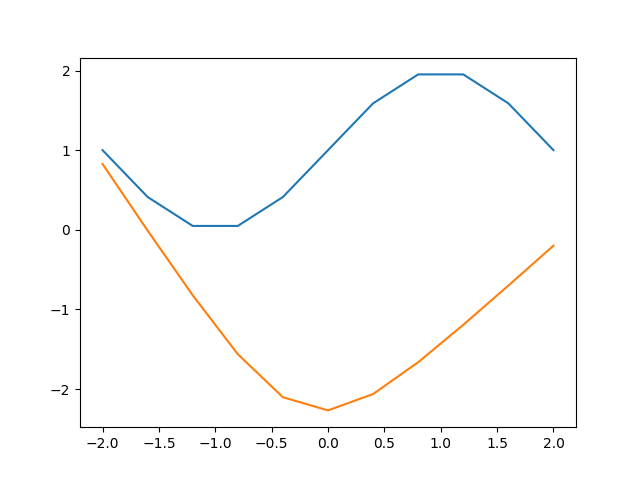
\includegraphics[width=6cm]{photos/1_001.png}
    \label{fig:2}
\end{figure}
Final weight1: [0.030909503133541627, -3.1942548621059763, -3.1069772191111356]\\ and bias1: [0.5112930381588776, -0.0038236442505651244, -0.03493906158817512]\\
Final weight2: [0.7868737753116977, -0.6733869741641436, -0.6539490598958959]\\ and bias2: 1.1681376688809941\\
P0 is 0.8263888898491442 and is supposed to be 0.9999999999999999\\
P1 is -0.009524055853615154 and is supposed to be 0.41221474770752675\\
P2 is -0.8216509447115238 and is supposed to be 0.04894348370484636\\
P3 is -1.5610607586741283 and is supposed to be 0.04894348370484647\\
P4 is -2.1011380032554157 and is supposed to be 0.41221474770752686\\
P5 is -2.2665685056520224 and is supposed to be 1.0\\
P6 is -2.0612501510493635 and is supposed to be 1.5877852522924731\\
P7 is -1.6618523455024368 and is supposed to be 1.9510565162951536\\
P8 is -1.1922061417108392 and is supposed to be 1.9510565162951536\\
P9 is -0.6996341191567705 and is supposed to be 1.5877852522924734\\
P10 is -0.19883030363382093 and is supposed to be 1.0000000000000002\\~\\
Learning rate = 0.001 and s=15\\
\begin{figure}[htp]
    \centering
    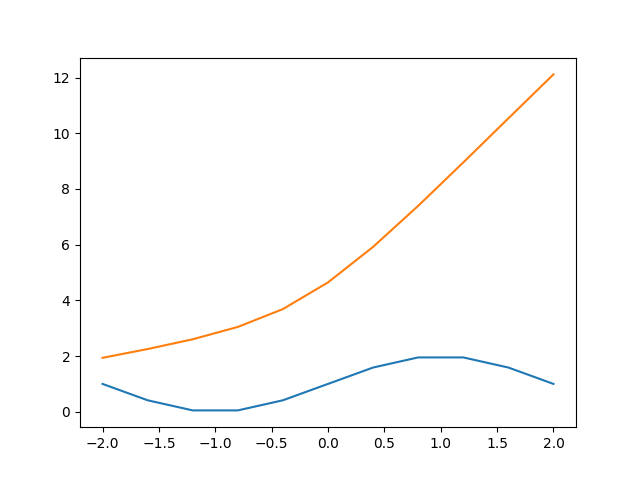
\includegraphics[width=6cm]{photos/2_001.png}
    \label{fig:2}
\end{figure}
Final weight1: [0.44248942488399756, 2.192577697977375, -2.9334139200837996, 0.023921515983921348, 0.1655817134382285, 0.08042321033838204, -0.25129977565460937, -1.7874009468671817, -0.9457353201443084, -0.05928499625125257, 1.2991168623567368, -0.4632036069582728, 1.0495255718224887, 0.13163840730061563, 0.20572166694019547]\\ and bias1: [-0.11734813295953414, 0.11293384881877229, 0.04977567352124146, 0.18966767919722374, -0.15091223854548963, 0.4146491855413997, 0.4510993079333351, 0.01584086676386032, 0.15350363148328103, -0.208116011985671, -0.02202720588175104, 0.28334630953654366, 0.19555675069896544, 0.3271045368598385, 0.3408128065616652]\\
Final weight2: [-0.047223304497623776, 0.22556669924561606, -0.8016135689844859, -0.02377623811570163, -0.2646619467263139, 0.003107406186166055, 0.5277092052373649, -0.25001679839177476, 0.15481301876079062, 0.49869553562195834, 0.3767325473095455, 0.5162848333788569, 0.17864500535177347, 0.08628723979248827, 0.46686824344210454]\\ and bias2: 0.04223447251335259\\
P0 is 1.9366610083957623 and is supposed to be 0.9999999999999999\\
P1 is 2.251975615154788 and is supposed to be 0.41221474770752675\\
P2 is 2.6024578046802644 and is supposed to be 0.04894348370484636\\
P3 is 3.0456421915182776 and is supposed to be 0.04894348370484647\\
P4 is 3.686633485414877 and is supposed to be 0.41221474770752686\\
P5 is 4.644236623691551 and is supposed to be 1.0\\
P6 is 5.920127967409252 and is supposed to be 1.5877852522924731\\
P7 is 7.392649070245966 and is supposed to be 1.9510565162951536\\
P8 is 8.950781625121916 and is supposed to be 1.9510565162951536\\
P9 is 10.533635746706944 and is supposed to be 1.5877852522924734\\
P10 is 12.111946940528163 and is supposed to be 1.0000000000000002\\~\\
Learning rate = 0.005 and S=3\\
\begin{figure}[htp]
    \centering
    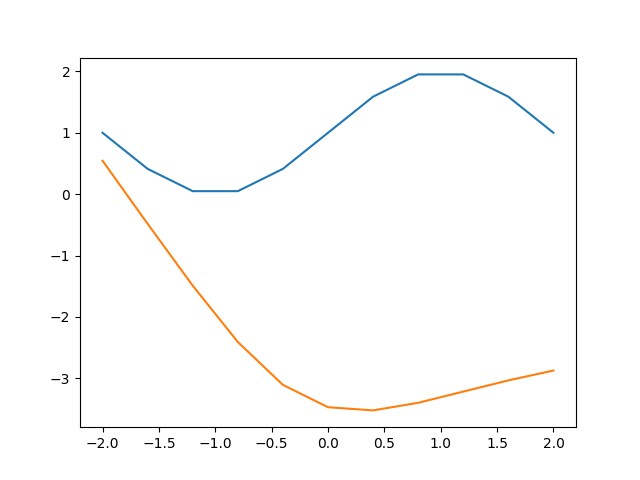
\includegraphics[width=6cm]{photos/1_005.png}
    \label{fig:2}
\end{figure}
Final weight1: [-0.8419387318381734, -2.469628232488532, -0.6625817894012812]\\ and bias1: [0.05687613055865347, -0.12860465010128191, 0.29883535110650133]\\
Final weight2: [0.21118944892587627, -1.6425329669736575, 0.5158409399669326]\\ and bias2: 1.3970208646859419\\
P0 is 0.5445437204361546 and is supposed to be 0.9999999999999999\\
P1 is -0.4828967327193102 and is supposed to be 0.41221474770752675\\
P2 is -1.4907611273684096 and is supposed to be 0.04894348370484636\\
P3 is -2.4079381121750125 and is supposed to be 0.04894348370484647\\
P4 is -3.1069389266087093 and is supposed to be 0.41221474770752686\\
P5 is -3.4706978148065857 and is supposed to be 1.0\\
P6 is -3.52266845128195 and is supposed to be 1.5877852522924731\\
P7 is -3.3989140165481033 and is supposed to be 1.9510565162951536\\
P8 is -3.216297011566445 and is supposed to be 1.9510565162951536\\
P9 is -3.033802588854829 and is supposed to be 1.5877852522924734\\
P10 is -2.8733159094187606 and is supposed to be 1.0000000000000002\\
Learning rate = 0.005 and S=15\\
\begin{figure}[htp]
    \centering
    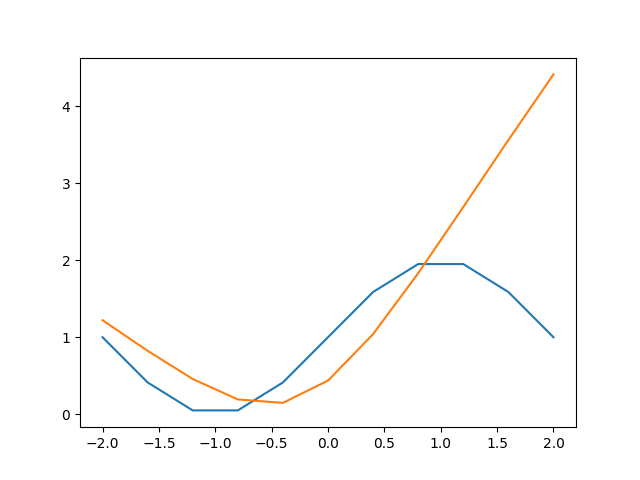
\includegraphics[width=6cm]{photos/2_005.png}
    \label{fig:2}
\end{figure}
Final weight1: [1.0483386583475927, -0.027818322420441088, 0.20730636410898232, -2.641580661484995, -0.32305620552702596, 0.03227842637125662, -0.6575980949914932, -0.1550287283973066, 1.4421031210482036, -0.09104542725601783, 0.20837479838020448, -0.1008441735787519, -0.21982411464533727, -2.019067621503454, 0.001870705741622904]\\ and bias1: [-0.3061649971615442, 0.30186652366327255, -0.12069880594199672, -0.09491564068117862, 0.10004960663062432, -0.08161690398191108, 0.22812032856039874, 0.4319525950320058, 0.2483794180191233, 0.4125995970135096, -0.23510101808461378, 0.26996947956350886, -0.31118732117359915, -0.04376261069444169, -0.25878865930926376]\\
Final weight2: [-0.28748440801038627, 0.45695770488490806, 0.34104022389889865, -1.025286634976018, 0.3678096786267325, -0.3604502273783705, 0.2399336097050874, 0.01190148666249783, 0.3105063161071186, -0.13555167548617963, 0.04821312624796542, 0.03129651439459619, 0.5224922001833565, -0.4965958108634263, 0.47139208311967684]\\ and bias2: 0.7317846751523781\\
P0 is 1.220706150009886 and is supposed to be 0.9999999999999999\\
P1 is 0.8234000579309669 and is supposed to be 0.41221474770752675\\
P2 is 0.4569809513973019 and is supposed to be 0.04894348370484636\\
P3 is 0.19149662825713823 and is supposed to be 0.04894348370484647\\
P4 is 0.14686202679453045 and is supposed to be 0.41221474770752686\\
P5 is 0.43592815152071773 and is supposed to be 1.0\\
P6 is 1.0405847184060888 and is supposed to be 1.5877852522924731\\
P7 is 1.8311735605021464 and is supposed to be 1.9510565162951536\\
P8 is 2.692391976954826 and is supposed to be 1.9510565162951536\\
P9 is 3.5625317272403487 and is supposed to be 1.5877852522924734\\
P10 is 4.4158928630509475 and is supposed to be 1.0000000000000002\\
Learning rate = 0.01 and S=3\\~\\
\begin{figure}[htp]
    \centering
    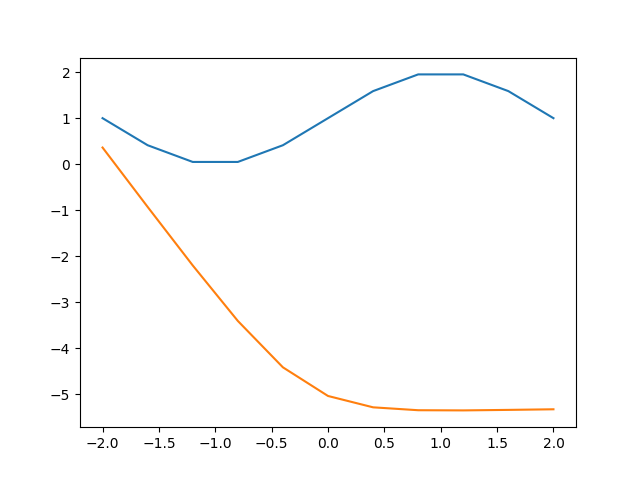
\includegraphics[width=6cm]{photos/1_01.png}
    \label{fig:2}
\end{figure}
Final weight1: [-3.2747628057401945, -0.6556448833569682, -0.6655380952383398]\\ and bias1: [-0.04502160721259928, 0.22332333021315504, -0.4540506384021959]\\
Final weight2: [-1.3340811051148649, 0.08634553188202508, -0.047309571489522126]\\ and bias2: 1.6291113423259438\\
P0 is 0.36190769225761305 and is supposed to be 0.9999999999999999\\
P1 is -0.9280289346499493 and is supposed to be 0.41221474770752675\\
P2 is -2.199637366917776 and is supposed to be 0.04894348370484636\\
P3 is -3.405271893522561 and is supposed to be 0.04894348370484647\\
P4 is -4.413662097507572 and is supposed to be 0.41221474770752686\\
P5 is -5.036090943009504 and is supposed to be 1.0\\
P6 is -5.282819361806901 and is supposed to be 1.5877852522924731\\
P7 is -5.345772146802508 and is supposed to be 1.9510565162951536\\
P8 is -5.349561788926244 and is supposed to be 1.9510565162951536\\
P9 is -5.3384909568011505 and is supposed to be 1.5877852522924734\\
P10 is -5.3253510574372855 and is supposed to be 1.0000000000000002\\
Learning rate = 0.01 and S=15\\~\\
\begin{figure}[htp]
    \centering
    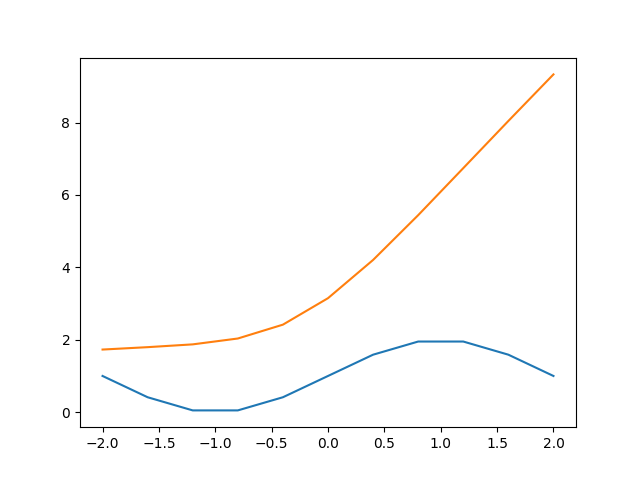
\includegraphics[width=6cm]{photos/2_01.png}
    \label{fig:2}
\end{figure}
Final weight1: [-2.0237520231170962, -0.09893143399059656, -0.21210133740179446, 0.016536964024686667, -2.4601126708409984, -0.024688676945908556, 0.4158409485327284, 1.6603391162739862, 1.1596126677694492, 0.7278911198560799, 2.615943128110069, -0.03841717876716053, -0.022914155563302018, 0.2468067593753753, 0.23828711324676885]\\ and bias1: [-0.3259279390668322, 0.41086447512186985, 0.010480276465058091, -0.26393996984709106, -0.10419349348505465, 0.28243426993717424, -0.27078446052594146, 0.15880785853913773, 0.34905474581804186, -0.1631155521688279, 0.14511728897520065, 0.3697126022661095, 0.24599762409379913, -0.4097029510828328, 0.4311591216569938]\\
Final weight2: [-0.2534172608951247, 0.5990518993465422, 0.680319420729582, -0.40295521635078824, -0.7576281623173399, 0.32792856917174046, -0.10189424164139978, -0.029459129632529314, -0.39030433536374115, -0.16110986952858639, 0.7892000849571653, 0.322811868474445, -0.11903385661336525, 0.3255190160450032, 0.2775181251259697]\\ and bias2: 0.2679078651681681\\
P0 is 1.7296084544589791 and is supposed to be 0.9999999999999999\\
P1 is 1.7957283265393613 and is supposed to be 0.41221474770752675\\
P2 is 1.872737787166379 and is supposed to be 0.04894348370484636\\
P3 is 2.034560178740187 and is supposed to be 0.04894348370484647\\
P4 is 2.4173562964327773 and is supposed to be 0.41221474770752686\\
P5 is 3.1486176744669923 and is supposed to be 1.0\\
P6 is 4.204385448102281 and is supposed to be 1.5877852522924731\\
P7 is 5.441429307396668 and is supposed to be 1.9510565162951536\\
P8 is 6.74042640905029 and is supposed to be 1.9510565162951536\\
P9 is 8.04340414023412 and is supposed to be 1.5877852522924734\\
P10 is 9.32952197475456 and is supposed to be 1.0000000000000002\\~\\
By the results from the learning rates we used,the value of the learning rate seems to be more reliable between the values of 0.1 and 0.001 because the g(p) function changes periodically and its' results are between 0 and 2.Lower learning rates help the training by changing the direction of the graph with more ease.  
\section{.}
Dropout probability = 0.10\\
\begin{figure}[htp]
    \centering
    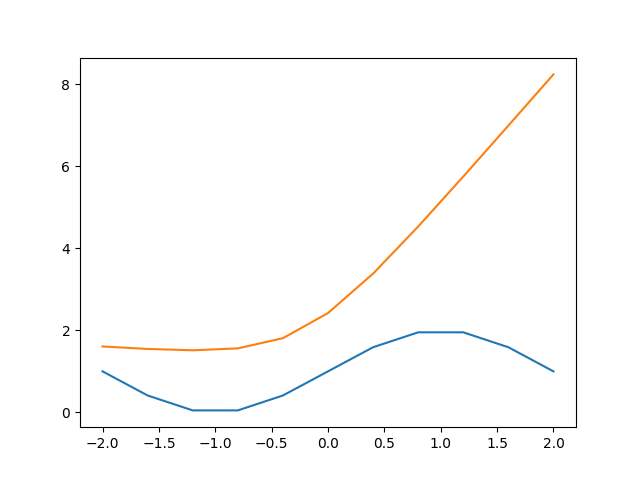
\includegraphics[width=6cm]{photos/ask7_10.png}
    \label{fig:2}
\end{figure}
Final weight1: [-2.59910509  0.11120802  0.04913053 -0.01710935 -0.40061256 -0.17218889
  0.         -0.10881888  0.05121299 -0.07120143 -0.21352516 -1.13821909
  0.          2.19343773  3.28428206]\\ and bias1: [ 0.02125911  0.09966034 -0.13790664  0.25835404 -0.35902373 -0.40731497
  0.          0.08744258  0.06730358  0.39121647  0.35541087 -0.21745325
  0.          0.04988636  0.07497568]\\
Final weight2: [-0.09375145 -0.26012935 -0.33176239  0.3031241  -0.06749578 -0.07396368
 -0.40910055  0.4595959   0.50765136  0.         -0.06594695  0.
 -0.14486669  0.31212735  0.94427507]\\ and bias2: 0.3888552378385044\\
P0 is 1.6063565932441717 and is supposed to be 0.9999999999999999\\
P1 is 1.5465368957975516 and is supposed to be 0.41221474770752675\\
P2 is 1.5135645553075916 and is supposed to be 0.04894348370484636\\
P3 is 1.5597572126274655 and is supposed to be 0.04894348370484647\\
P4 is 1.8085356608153844 and is supposed to be 0.41221474770752686\\
P5 is 2.420116840610599 and is supposed to be 1.0\\
P6 is 3.381586799543923 and is supposed to be 1.5877852522924731\\
P7 is 4.5285037980884715 and is supposed to be 1.9510565162951536\\
P8 is 5.746222955758188 and is supposed to be 1.9510565162951536\\
P9 is 6.98740151229165 and is supposed to be 1.5877852522924734\\
P10 is 8.235041498629453 and is supposed to be 1.0000000000000002\\

Dropout probability = 0.25\\
\begin{figure}[htp]
    \centering
    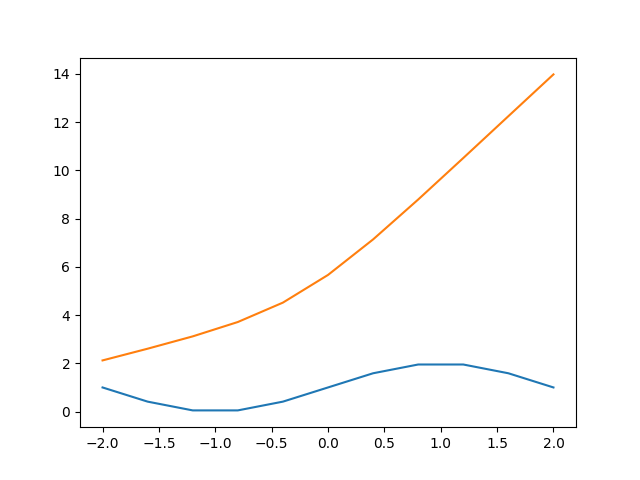
\includegraphics[width=6cm]{photos/ask7_25.png}
    \label{fig:2}
\end{figure}
Final weight1: [ 8.58672372e-01  0.00000000e+00  3.39537126e-02  0.00000000e+00
  3.25577600e-01  2.07978851e+00  0.00000000e+00 -1.64843112e-03
 -2.23555589e+00  2.71709630e+00  1.31452509e+00 -1.19593827e+00
  2.10880056e-01 -7.51945555e-02  0.00000000e+00]\\ and bias1: [-0.1690654   0.          0.27909064  0.         -0.18602904  0.03264184
  0.          0.01307758 -0.10866247  0.08776054 -0.09998297 -0.03050814
 -0.15209358  0.09353     0.        ]\\
Final weight2: [-0.45340106  0.55331627  0.         -0.1090509   0.34532304  0.08985712
  0.          0.31457253 -0.          1.41793166 -0.08810215  0.
  0.2317704   0.08018592 -0.15165098]\\ and bias2: -0.13774154918341364\\
P0 is 2.1203701555272065 and is supposed to be 0.9999999999999999\\
P1 is 2.606043771664603 and is supposed to be 0.41221474770752675\\
P2 is 3.116716283593564 and is supposed to be 0.04894348370484636\\
P3 is 3.7118037127905557 and is supposed to be 0.04894348370484647\\
P4 is 4.515802689577027 and is supposed to be 0.41221474770752686\\
P5 is 5.662412330515885 and is supposed to be 1.0\\
P6 is 7.134933289133754 and is supposed to be 1.5877852522924731\\
P7 is 8.788521787398686 and is supposed to be 1.9510565162951536\\
P8 is 10.507708563296589 and is supposed to be 1.9510565162951536\\
P9 is 12.241272140607023 and is supposed to be 1.5877852522924734\\
P10 is 13.973416628346884 and is supposed to be 1.0000000000000002\\

Dropout probability = 0.50\\
\begin{figure}[htp]
    \centering
    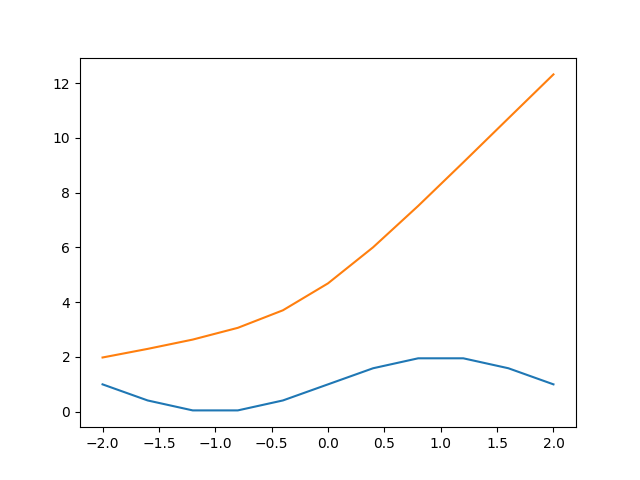
\includegraphics[width=6cm]{photos/ask7_50.png}
    \label{fig:2}
\end{figure}
Final weight1: [ 1.89135572  0.          0.          0.          0.          2.37380589
  0.         -1.61275657  0.          0.25219742 -0.35666342 -3.05603642
  0.          2.71251341  0.        ] \\and bias1: [-0.09784551  0.          0.          0.          0.          0.13734658
  0.         -0.10566741  0.          0.11077245  0.04867221  0.01692556
  0.          0.05744437  0.        ]\\
Final weight2: [-0.00000000e+00 -1.16140799e-03 -0.00000000e+00 -0.00000000e+00
 -2.08932055e-02 -0.00000000e+00  3.63927823e-01 -1.80894902e-01
 -0.00000000e+00 -0.00000000e+00  6.00020116e-01 -0.00000000e+00
 -0.00000000e+00  1.33952651e+00 -1.95809416e-01]\\ and bias2: 0.020152768895894554\\
P0 is 1.980419392484462 and is supposed to be 0.9999999999999999\\
P1 is 2.294898766470035 and is supposed to be 0.41221474770752675\\
P2 is 2.634825090047943 and is supposed to be 0.04894348370484636\\
P3 is 3.063495983069266 and is supposed to be 0.04894348370484647\\
P4 is 3.703926313288953 and is supposed to be 0.41221474770752686\\
P5 is 4.687589719848333 and is supposed to be 1.0\\
P6 is 6.0040720809547565 and is supposed to be 1.5877852522924731\\
P7 is 7.515050843947688 and is supposed to be 1.9510565162951536\\
P8 is 9.103515137911428 and is supposed to be 1.9510565162951536\\
P9 is 10.711685202576104 and is supposed to be 1.5877852522924734\\
P10 is 12.316275328055655 and is supposed to be 1.0000000000000002\\~\\

In addition to the previous exercise,the dropout technique gives more stability to the system results by reducing the nuber of weights. 
\newpage
\section{.}
\begin{figure}[htp]
    \centering
    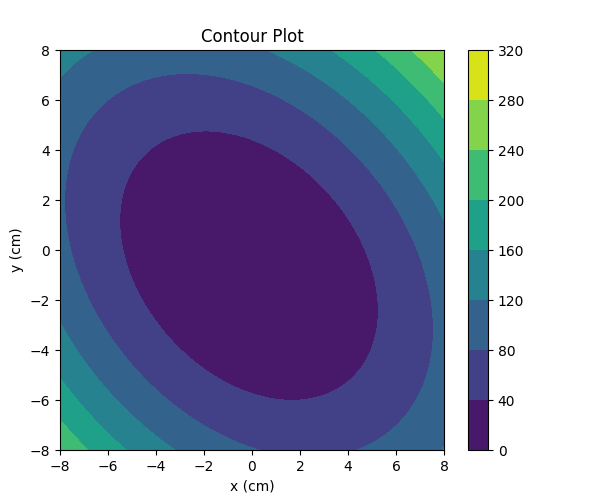
\includegraphics[width=7cm]{photos/8_contour.png}
    \label{fig:2}
\end{figure}
This is the contour plot of the F(x) function,we used python's matplotlib library in the file ask8.py that we added in the code folder.
\newpage
\section{.}
Adam with $\beta_1=0,\beta_2$ really close to 1 and a replacement of a by an annealed version $a_t=at^{-1/2}$,which is \\
\begin{figure}[htp]
    \centering
    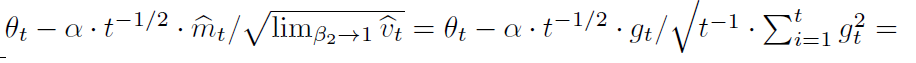
\includegraphics[width=10cm]{photos/1st_adam.png}
    \label{fig:2}
\end{figure}\\
\begin{figure}[htp]
    \centering
    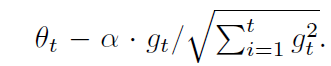
\includegraphics[width=4cm]{photos/2nd_adam.png}
    \label{fig:2}
\end{figure}\\
corresponds to Adagrad with $\beta_2$ converging to 1 from from bellow,and so 
\begin{figure}[htp]
    \centering
    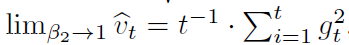
\includegraphics[width=6cm]{photos/2nd_adagrad.png}
    \label{fig:2}
\end{figure}\\
\newpage
\section{.}
\begin{figure}[htp]
    \centering
    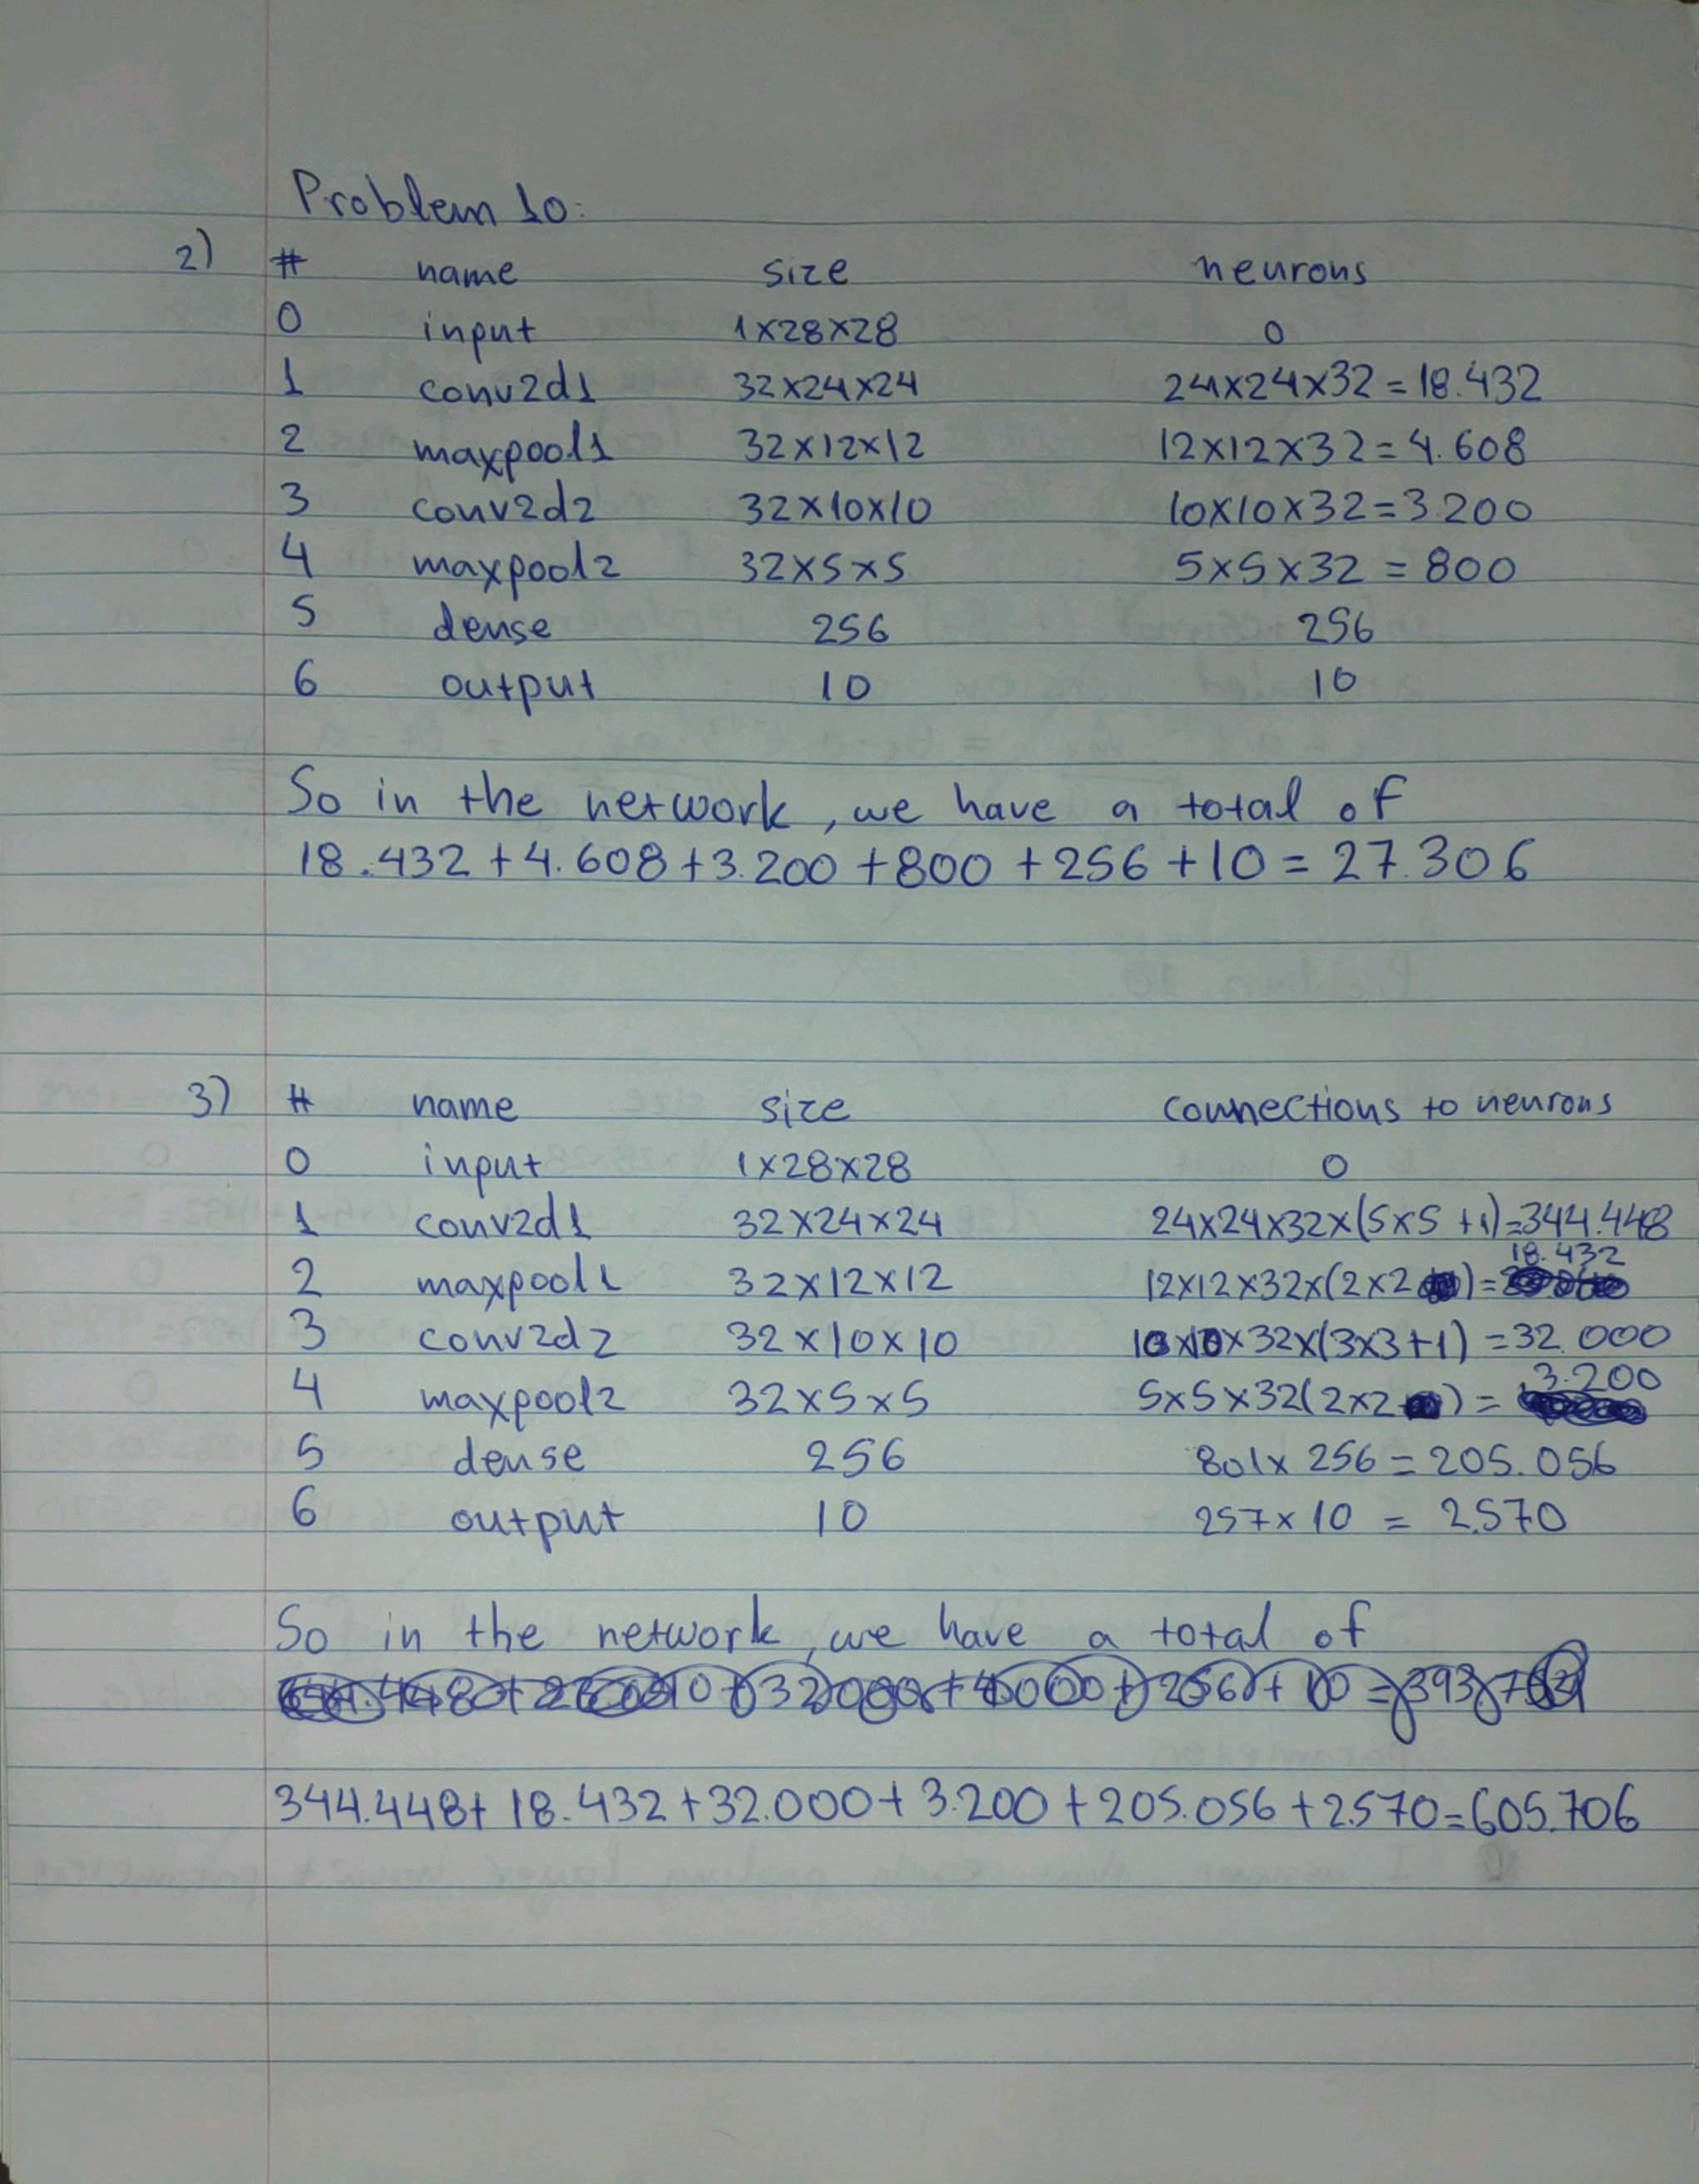
\includegraphics[width=11cm]{photos/10_1.jpg}
    \label{fig:2}
\end{figure}
\begin{figure}[htp]
    \centering
    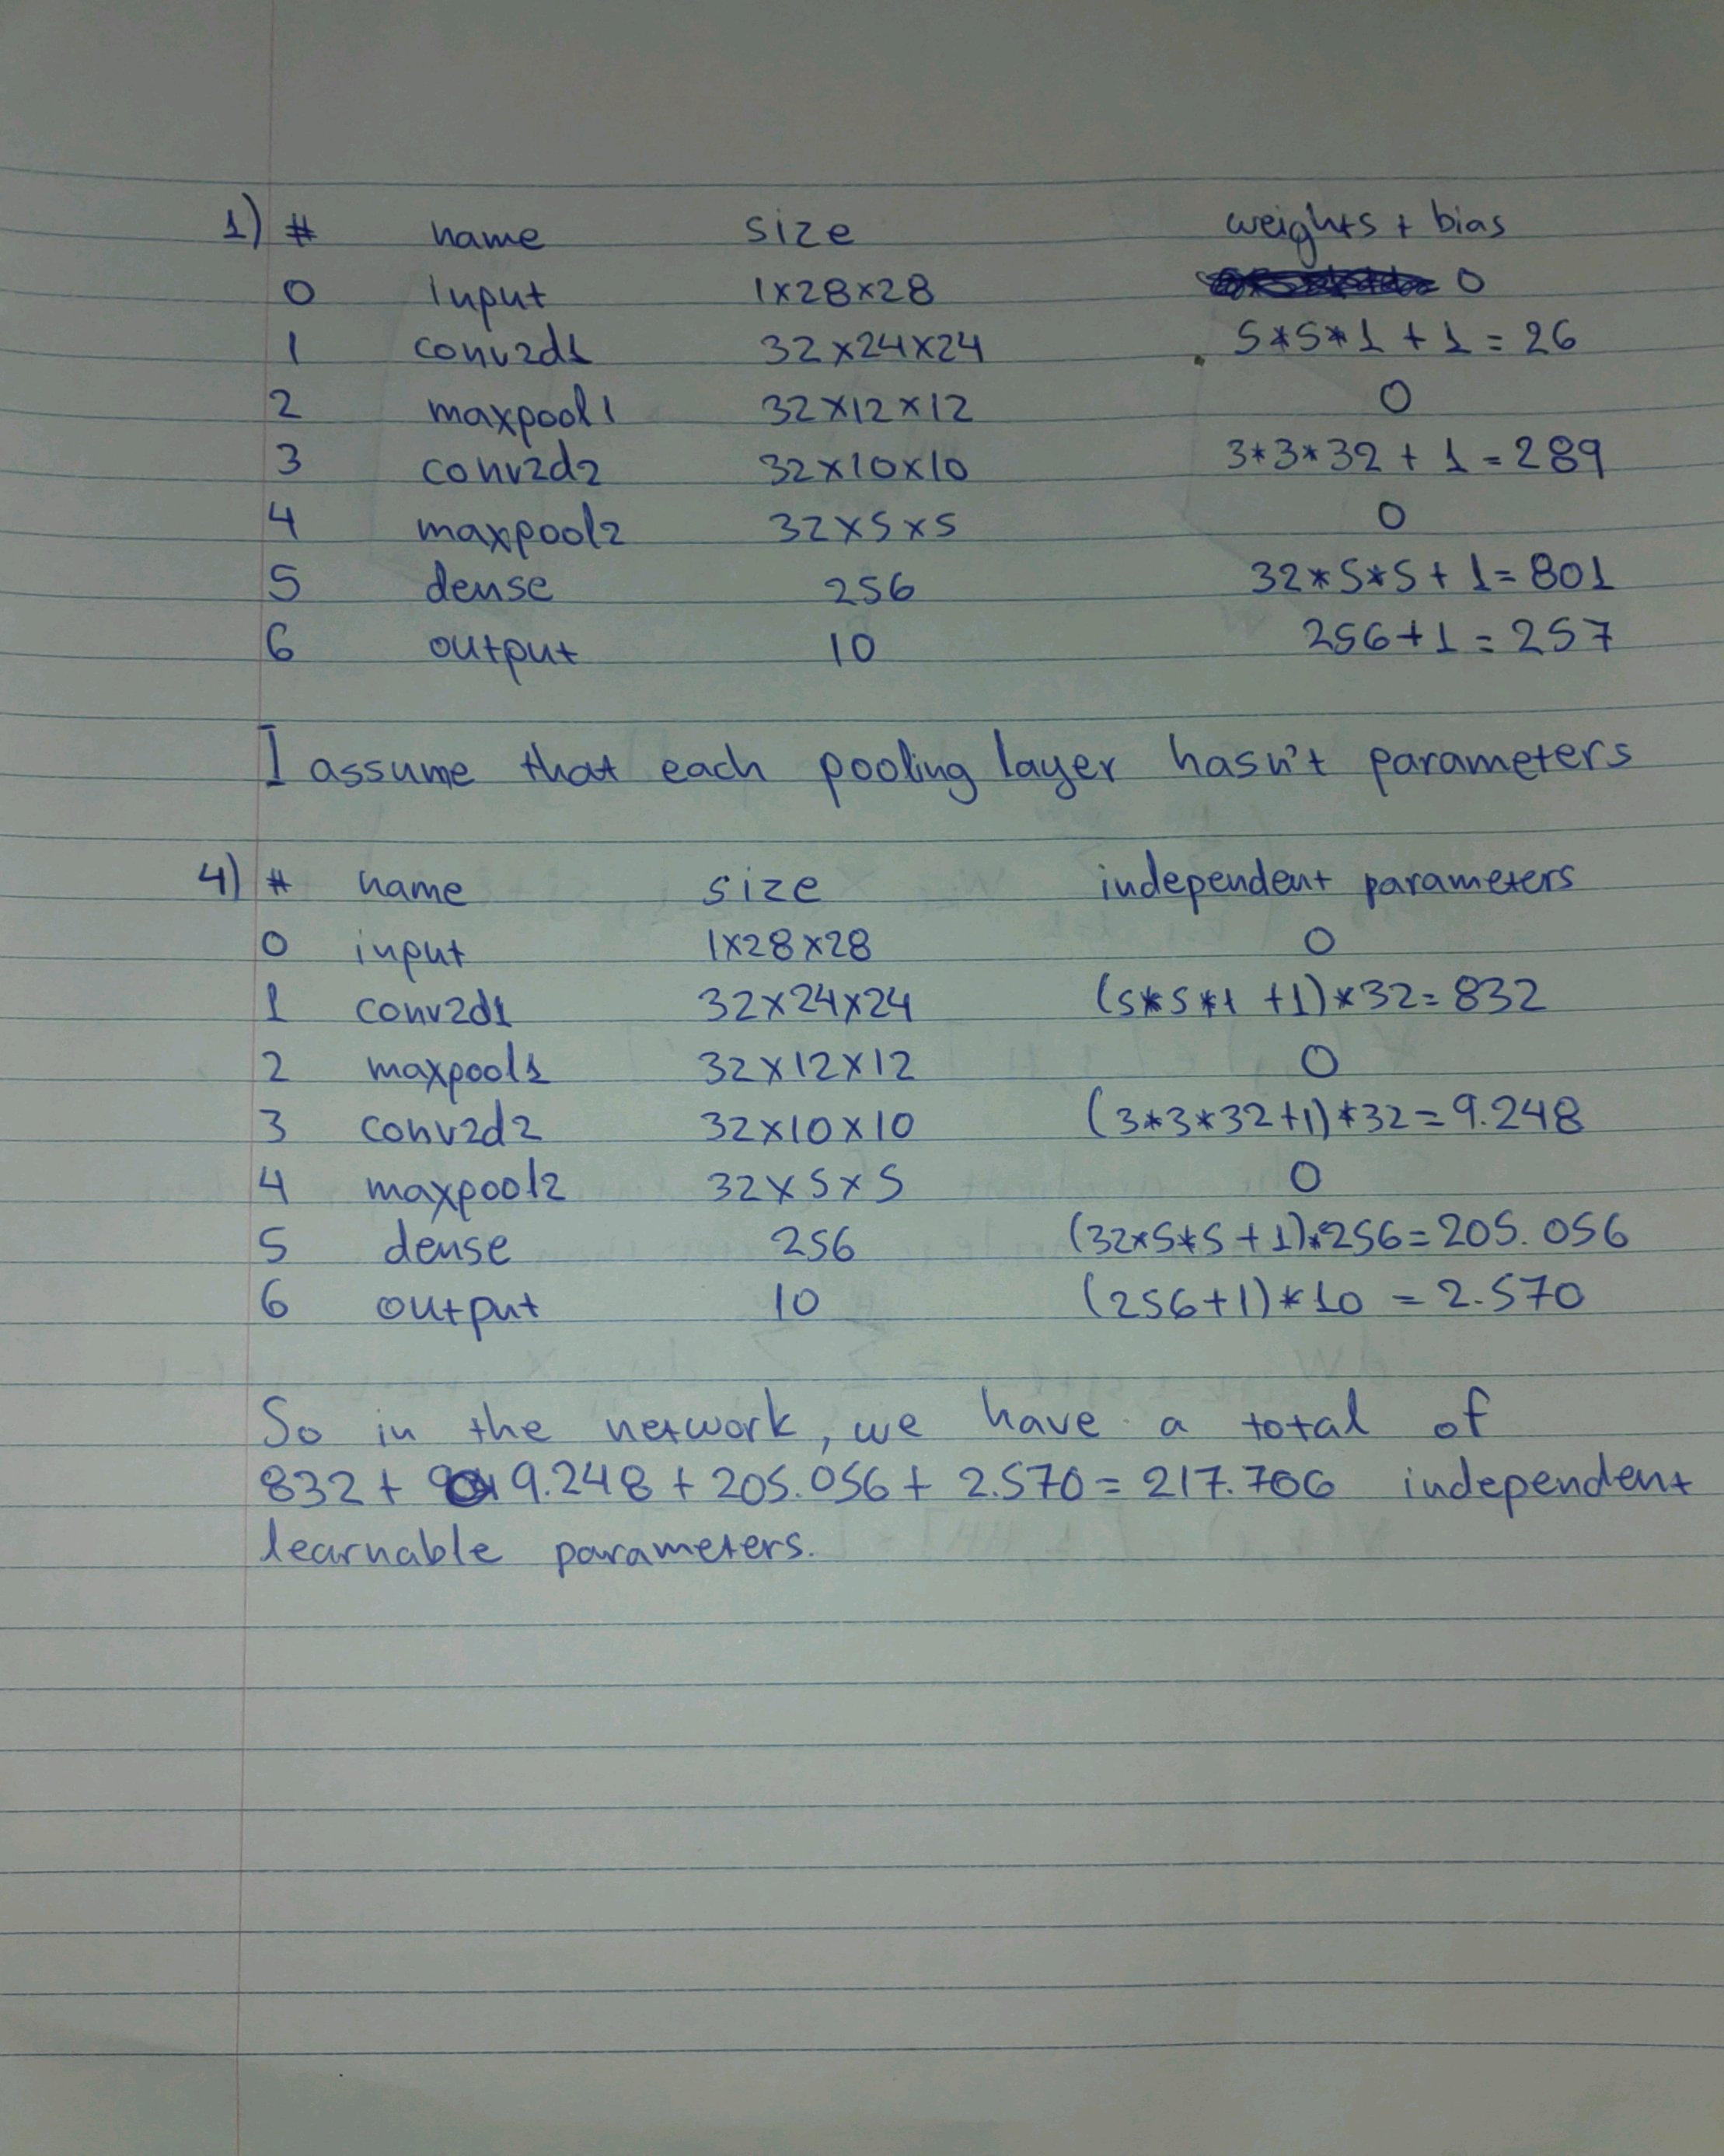
\includegraphics[width=11cm]{photos/10_2.jpg}
    \label{fig:2}
\end{figure}
\newpage
\section{.}

Input1:

\begin{tabular}{|p{0.2in}|p{0.2in}|p{0.2in}|p{0.2in}|p{0.2in}|p{0.2in}|p{0.2in}|p{0.2in}|p{0.2in}|p{0.2in}|p{0.2in}|p{0.2in}|} \hline 
0 & 0 & 0 & 0 & 1 & 1 & 1 & 1 & 0 & 0 & 0 & 0 \\ \hline 
\end{tabular}

Convolution with: 

\begin{tabular}{|p{0.3in}|p{0.3in}|p{0.3in}|} \hline 
-1 & 0 & 1 \\ \hline 
1 & 0 & -1 \\ \hline 
\end{tabular}



 

 Equals:

\begin{tabular}{|p{0.3in}|p{0.3in}|p{0.3in}|p{0.3in}|p{0.3in}|p{0.3in}|p{0.3in}|p{0.3in}|p{0.3in}|p{0.3in}|} \hline 
0 & 0 & 1 & 1 & 0 & 0 & -1 & -1 & 0 & 0 \\ \hline 
0 & 0 & -1 & -1 & 0 & 0 & 1 & 1 & 0 & 0 \\ \hline 
\end{tabular}

Max pooling with stride=2 and filter size=2:

  

\begin{tabular}{|p{0.5in}|p{0.5in}|p{0.5in}|p{0.5in}|p{0.5in}|} \hline 
0 & 1 & 0 & -1 & 0 \\ \hline 
0 & -1 & 0 & 1 & 0 \\ \hline 
\end{tabular}

 

 Convolution with:

\begin{tabular}{|p{0.4in}|p{0.4in}|p{0.4in}|} \hline 
-1 & 0 & 1 \\ \hline 
1 & 0 & -1 \\ \hline 
\end{tabular}



 Equals:  

\begin{tabular}{|p{0.5in}|p{0.5in}|p{0.5in}|} \hline 
0 & -4 & 0 \\ \hline 
\end{tabular}

 

 

 Fully connected layer:

\begin{tabular}{|p{0.4in}|p{0.4in}|} \hline 
4 & -4 \\ \hline 
\end{tabular}

 Sigmoid activation(1/(1+e${}^{-x}$))=

\begin{tabular}{|p{0.4in}|p{0.4in}|} \hline 
0.99 & 0.1 \\ \hline 
\end{tabular}\\
\\~\\

Input2:\\

\begin{tabular}{|p{0.2in}|p{0.2in}|p{0.2in}|p{0.2in}|p{0.2in}|p{0.2in}|p{0.2in}|p{0.2in}|p{0.2in}|p{0.2in}|p{0.2in}|p{0.2in}|} \hline 
1 & 1 & 1 & 1 & 0 & 0 & 0 & 0 & 1 & 1 & 1 & 1 \\ \hline 
\end{tabular}

Convolution with: 

\begin{tabular}{|p{0.3in}|p{0.3in}|p{0.3in}|} \hline 
-1 & 0 & 1 \\ \hline 
1 & 0 & -1 \\ \hline  
\end{tabular}

 Equals:

\begin{tabular}{|p{0.3in}|p{0.3in}|p{0.3in}|p{0.3in}|p{0.3in}|p{0.3in}|p{0.3in}|p{0.3in}|p{0.3in}|p{0.3in}|} \hline 
0 & 0 & -1 & -1 & 0 & 0 & 1 & 1 & 0 & 0 \\ \hline 
0 & 0 & 1 & 1 & 0 & 0 & -1 & -1 & 0 & 0 \\ \hline 
\end{tabular}\\
\\~

Max pooling with stride=2 and filter size=2:

  

\begin{tabular}{|p{0.5in}|p{0.5in}|p{0.5in}|p{0.5in}|p{0.5in}|} \hline 
0 & -1 & 0 & 1 & 0 \\ \hline 
0 & 1 & 0 & -1 & 0 \\ \hline 
\end{tabular}

 

 Convolution with:

\begin{tabular}{|p{0.4in}|p{0.4in}|p{0.4in}|} \hline 
-1 & 0 & 1 \\ \hline 
1 & 0 & -1 \\ \hline 
\end{tabular}



 Equals:  

\begin{tabular}{|p{0.5in}|p{0.5in}|p{0.5in}|} \hline 
0 & 4 & 0 \\ \hline 
\end{tabular}

 

 

 Fully connected layer:

\begin{tabular}{|p{0.4in}|p{0.4in}|} \hline 
-4 & 4 \\ \hline 
\end{tabular}

 Sigmoid activation(1/(1+e${}^{-x}$))=

\begin{tabular}{|p{0.4in}|p{0.4in}|} \hline 
0.1 & 0.99 \\ \hline 
\end{tabular}
\section{.}
\begin{figure}[htp]
    \centering
    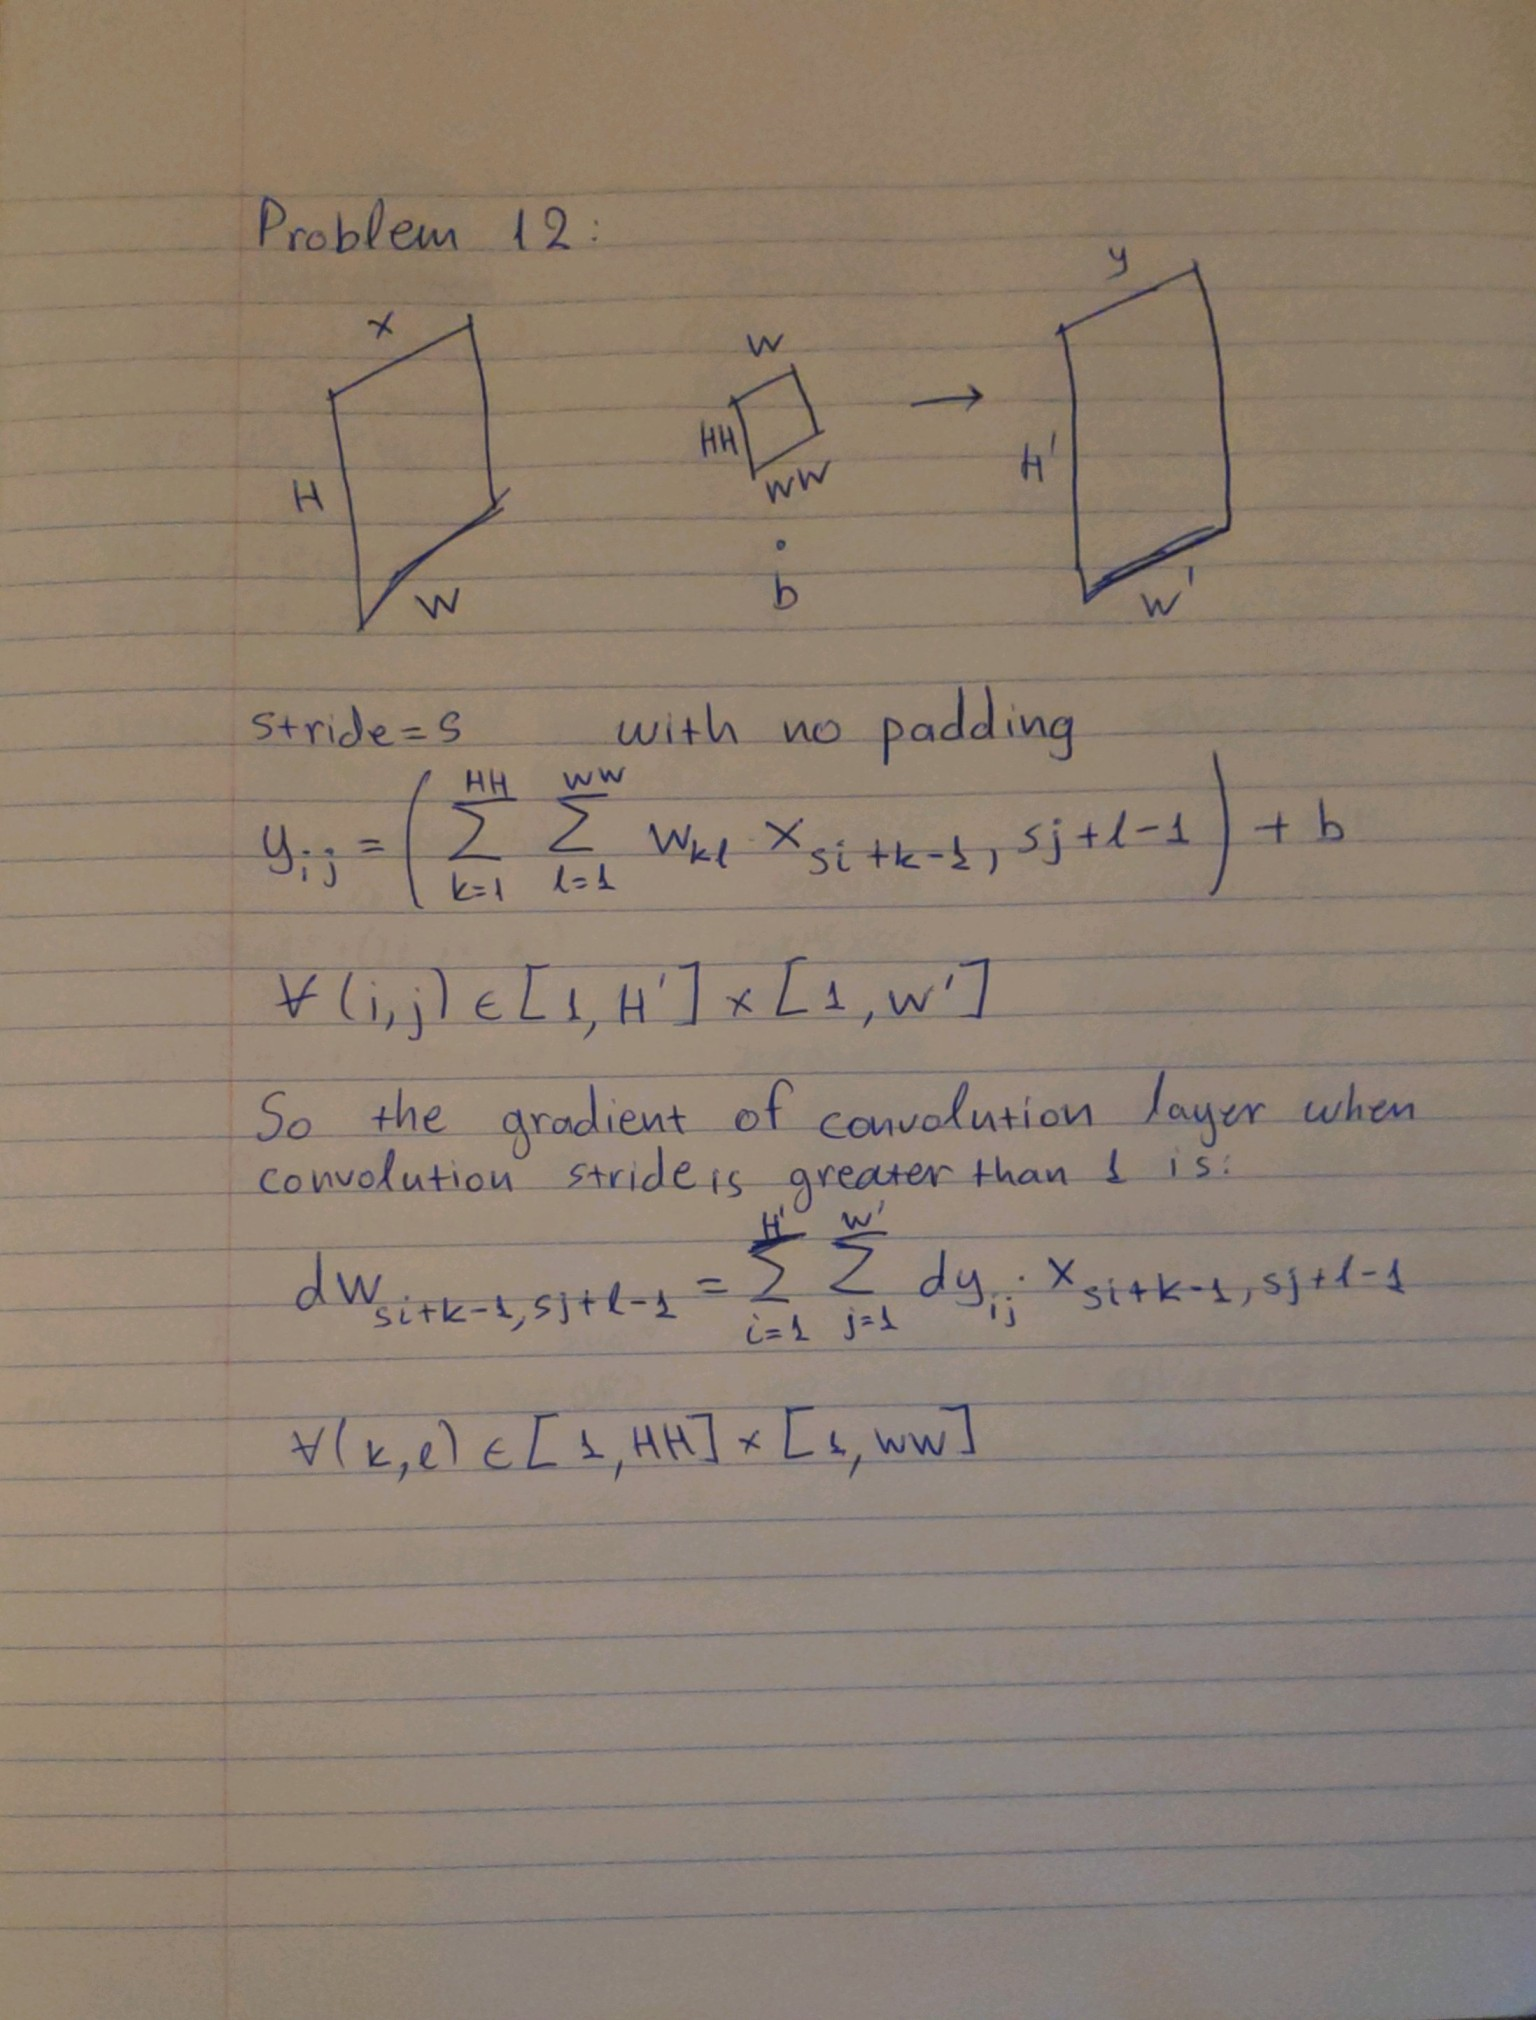
\includegraphics[width=11cm]{photos/12.jpg}
    \label{fig:2}
\end{figure}
\newpage
\section{.}
When the gradient includes overlapping regions with the same parameters, the gradients values from the source can be summed together, because the operations in the forward phase are also additions which means that $\frac{d}{dx}(y+z) = \frac{dy}{dx} + \frac{dz}{dx}$.This is exactly the case with max pooling as well.



\end{document}
